%!TEX encoding = UTF-8 Unicode 
\documentclass[12pt]{article} %try amsproc, amsart
\usepackage{geometry}                % See geometry.pdf to learn the layout options. There are lots.
\geometry{a4paper, margin=2.5cm}                   % ... or a4paper or a5paper or ... 
% \geometry{landscape}                % Activate for for rotated page geometry
\usepackage{graphicx}
\usepackage{amssymb}
\usepackage{amsmath}
\usepackage{amsthm}
\usepackage{setspace}
\setstretch{1.1}

\usepackage{hyperref}
\hyperbaseurl{}
\urlstyle{same}
\usepackage[ruled]{algorithm2e}
\newcommand{\lIfElse}[3]{\lIf{#1}{#2 \textbf{else}~#3}}

\usepackage{times}
\usepackage{letltxmacro}
\usepackage[shortlabels]{enumitem}
\usepackage{kotex}
\usepackage{fancyhdr}
\DeclareMathOperator*{\argmax}{arg\,max}
\DeclareMathOperator*{\argmin}{arg\,min}



% Language selector
\newif\ifEN
\ENtrue % Change to false to export Korean
%\ENfalse


\ifEN
{
\newtheorem{theorem}{Theorem}
\newtheorem{lemma}{Lemma}
\newtheorem{corollary}{Corollary}
\newtheorem{proposition}{Proposition}
\theoremstyle{definition}
\newtheorem{example}{Example}
\newtheorem{definition}{Definition}
\newtheorem{assumption}{Assumption}
\newtheorem{conjecture}{Conjecture}
}
\else {
\newtheorem{theorem}{정리}
\newtheorem{lemma}{기본정리}
\newtheorem{corollary}{따름정리}
\newtheorem{proposition}{제의}
\theoremstyle{definition}
\newtheorem{example}{예}
\newtheorem{definition}{정의}
\newtheorem{assumption}{가정}
\newtheorem{conjecture}{추측}
}
\fi

%\ifEN {} \else \renewcommand*{\proofname}{증명\@}  \fi



\pagestyle{fancy}
\renewcommand{\headrulewidth}{0pt}
\fancyhf{}
\rhead{Uncertainty in college admissions markets \\~}
\lhead{Max Kapur \\ \date{\today}}
\cfoot{\thepage}



\ifEN{ \title{College admissions markets with combinatorial preferences, constrained applications, and uncertainty} }
\else {\title{조합적 선호~\textbullet~지원 제한~\textbullet~불확실성을 고려한 대학 입시 시장}} \fi
\author{Max Kapur}
\date{\today}                % Activate to display a given date or no date

\begin{document}
\maketitle
\pagebreak

\tableofcontents
\pagebreak

\ifEN \section{Introduction}  \else \section{서론} \fi

\ifEN \section{Equilibrium model}  \else \section{균형 모형} \fi
\ifEN {
This study considers the efficiency of a college admissions market in which the following three features coincide:
\begin{enumerate}
\item \label{feat-combipref} Colleges have \emph{combinatorial} preferences over the composition of their entering class. 
\item \label{feat-uncertainty}There is \emph{uncertainty} in colleges’ preferences; that is, students have only probabilistic information about their admissions prospects at the time of application.
\item \label{feat-constrainedapp} Students are \emph{constrained} in the number of schools to which they can apply.  
\end{enumerate}
} \else {
본 연구는 다음과 같은 세가지 특징이 동시에 공존하는 대학 입학 시장을 고려한다.
\begin{enumerate}
\item 대학교는 신입생 집합에 대해 조합적인 선호순위를 가진다.
\item 학생이 지원할 수 있는 대학의 개수는 제한된다.
\item 대학의 선호순위는 불확실성을 포함한다. 즉, 지원 시에 학생의 합격 전망은 확률적인 정보로만 주어진다.
\end{enumerate}
} \fi
The model contains finite sets $\mathcal{S} = \{1 \dots n\}$ of students and $\mathcal{C} = \{1 \dots m\}$ of colleges. The name of student $i$ is $s_i$, and the name of college $j$ is $c_j$. 

Feature \ref{feat-combipref} says that each school has a preference order $\succapprox_j$ over the set of admitted-student cohorts. Note that $\succsim_j$ orders sets of \emph{admitted} students, with the understanding that only a subset of admits will actually enroll at the college. The college-specific optimization problem that produces $\succapprox_j$ is considered exogenous to our model. This assumption is reasonable because in this model, students' preferences are deterministic. 

Feature \ref{feat-uncertainty} arises in real admissions markets because there is asymmetry in the information that students have about themselves and the information that colleges collect about students in the application process. For example, students may have a rough idea of the quality of their personal essay, but the college's evaluation of the same will depend on the biases and mood of the reader. We model this asymmetry by regarding each $\succapprox_j$ as a random variable whose space is $2^{\mathcal{S}}!$. Specific realizations of $\succapprox_j$ are denoted $\succsim_j$. Notice that this definition alone does not impose any constraint on whether it is students who possess complete information about their qualifications and colleges who add measurement noise, or vice-versa. However, the following assumption (which greatly simplifies the subsequent analysis of student utility) implies that the noise is added by the colleges:
\begin{assumption} \label{preforderdrawnindep}
For two colleges $c_j$ and $c_{j'}$, $\succapprox_j$ is statistically independent of $\succapprox_{j'}$. 
\end{assumption}

Now we can specify the admissions procedure. First, students submit applications to a subset of colleges. Let $\mathcal{X}_i$ denote the set of schools to which $s_i$ applies. Next, each school draws a realization of its preference order $\succapprox_j$ and applies it to the set of applicants to determine which students to admit. Thus, when student $i$ applies to $c_j$, her admissions outcome is determined entirely by two variables: first, the set of applicants with whom she must compete; and second, the realization $\succsim_j$ of $c_j$’s preference order. In our model, the distribution of $\succapprox$ is exogenized. Therefore, student $i$’s \emph{admissions probability} can be expressed as a function of her peers’ application decisions.
\begin{assumption}[Existence of $f(\cdot)$]
Let $\mathcal{X}_{\setminus i}$ denote the application decisions of students other than $s_i$. Then
\begin{equation}
f_{ij}(\mathcal{X}_{\setminus i}) = \operatorname{Pr}\left[\;\parbox{23em}{$s_i$ admitted to $c_j$~\textbar~\\$s_i$ applies to $c_j$ and others’ application decisions are $\mathcal{X}_{\setminus i}$}\;\right] \in [0, 1]
\end{equation}
\end{assumption}

%\begin{assumption}[$c_1$ fills capacity] \label{c1fillcap}
%\begin{equation}
%|\{i' \neq i : j \in \mathcal{X}_{i'}\}| < q \implies f_{ij}(\mathcal{X}_{\setminus i}) = 1
%\end{equation}
%\end{assumption}
Going forward, we interact with the distributions of the random variables $\succapprox_j$ primarily via the function $f(\cdot)$. However, it is worth bearing in mind that $f_{.j}$ is a low-dimension projection of $c_j$'s true preference distribution. For example, suppose that $n=4$, $q=2$, and when all four students apply to $c_j$, $f_{.j} = (\tfrac{1}{2}, \tfrac{1}{2}, \tfrac{1}{2}, \tfrac{1}{2})$. This could mean that $c_j$ prefers all admitted-student cohorts with equal probability, or it could mean that $c_j$'s preferred cohort is $\{s_1, s_2\}$ with probability $1/2$ and $\{s_3, s_4\}$ with probability $1/2$. 

We model feature \ref{feat-constrainedapp} by allowing each student to apply to only $h$ colleges. Let $t_{ij}$ denote the utility that $s_i$ receives from attending $c_j$.  Assume that students receive zero utility if they do not attend college. Then we regard the expected utility associated with the application portfolio $\mathcal{X}_i$ as the value it provides the student.
\begin{definition}[Portfolio valuation function]
\begin{equation} \label{portfoliovaluationfn}% can expand here
v_i(\mathcal{X}_i) = \operatorname{E}\left[\max_{j \in \mathcal{X}_i }\{\text{$t_{ij}$~\textbar~$s_i$ admitted to $c_j$}\}\right]
\end{equation}
\end{definition}

The optimal application portfolio for $s_i$ is a set of $h$ schools that maximizes $v_i(\mathcal{X}_i)$. A polynomial-time algorithm for this combinatorial optimization problem is provided in \S\ref{optimalcollegeappstrat}.

If there are multiple optimal portfolios, then $s_i$ may elect to choose randomly among them. In fact, $s_i$ may find it strategically advantageous to do so. Thus, in the broadest conception, $s_i$'s decision variable is a probability vector $x_{i.}$ over the $\binom{m}{h}$ possible portfolios. We will refer to $x_{i.}$ as $s_i$'s \emph{application probability vector}, and regard each student's expected portfolio valuation as her utility function.
\begin{definition}[Student utility function]
The function
\begin{equation} \label{mixedstrategystudentutility}
u_i(x_{i.}) = \sum\nolimits_{l=1}^{\binom{m}{h}} v_i(\mathcal{X}_l) x_{il}
\end{equation}
is called student $s_i$'s \emph{utility function}, where $l$ is an index of the possible $h$-school application portfolios and $x_{il}$ is the probability that $s_i$ applies to the schools in $\mathcal{X}_l$,
\end{definition}
Now we are ready to define the market equilibrium.
\begin{definition}[Nash equilibrium]
The matrix of application probability vectors $x$, where $x_{il}$ represents the probability that $s_i$ applies to the $h$-school subset indicated by $l$, is said to be a (mixed-strategy) \emph{Nash equilibrium} if 
\begin{equation}
x_{i.} \in \argmax_{x_{i.}} \left\{ u_i(x_{i.}) : x_{il} \in [0, 1], \sum\nolimits_{l=1}^{\binom{m}{h}} x_{il} = 1 \right\},\quad \forall i \in \mathcal{S}
\end{equation}
If, furthermore, $x_{il} \in \{0, 1\}$ for all $i$ and $l$, then $x$ is called a \emph{pure-strategy} (Nash) equilibrium.
\end{definition}



%Consider the application portfolio optimization problem faced by students. Because student $s_i$'s expected utility function \eqref{mixedstrategystudentutility} is linear in $x_{il}$, there always exists a pure strategy application probability vector among the set of optima. This alone does not guarantee the existence of a pure-strategy \emph{equilibrium}, because $s_i$'s choice to play a pure strategy rather than a mixed strategy may create the opportunity for another student to improve her expected payoff. However, in a large market, the effect of one student's strategy on the values of $f(\mathcal{X})$ is quite small, as expressed in the following conjecture:
%\begin{conjecture}[Existence of approximate pure-strategy equilibrium]
%Every market admits at least one $\varepsilon$-approximate pure-strategy equilibrium. That is, every market admits a set of pure strategies such that each student's utility is within $\varepsilon$ of the optimum achievable in mixed strategies, where $\varepsilon \in O(1/ nm)$.
%\end{conjecture}
%This means that we can restrict our attention to pure strategies. But solving the portfolio optimization problem over pure strategies is relatively simple.

























\ifEN \section{The optimal college application strategy}  \else \section{최적 대학 지원 전략} \fi \label{optimalcollegeappstrat}
In this section, we consider the optimal college application strategy for a single student. As Chao (2014) remarked, this represents a somewhat subtle portfolio optimization problem. The traditional Markowitz model trades off the expected value across all assets with a risk term, obtaining a concave maximization problem with linear constraints. But college applicants maximize the observed value of their \emph{best} asset: If a student is admitted to her $j$th choice, then she is indifferent to whether or not she gets into her $(j+1)$th choice. As a result, the valuation function that students maximize is \emph{convex} in the expected utility associated with individual applications. Risk management is implicit in the college application problem because, in a typical admissions market, college preferability is negatively correlated with competitiveness. Thus, students must negotiate a tradeoff between highly attractive, selective “reach schools” and less preferable “safety schools” where admission is a safer bet. Finally, the combinatorial nature of the college application problem makes it difficult to solve using the gradient-based techniques used in continuous portfolio optimization.

Chao estimated her model (which considers application as a \emph{cost} rather than a constraint) by clustering the schools so that $m=8$, a scale at which enumeration is possible. However, subject to certain assumptions on the quality of the data available to students in their decisionmaking process, an optimal application portfolio for a single student can be computed in time polynomial in $h$ and $m$, as we show presently.

As this section considers a single student’s optimization problem, we drop subscripts where appropriate. 

% Nestedness property and paper

\ifEN \subsection{Problem formulation}  \else \subsection{모형화} \fi
Consider a college admissions market with $m$ schools, $\mathcal{C} = \{ 1 \dots m\}$. The $j$th school is named $c_j$. By government regulation, students are allowed to apply to no more than $h$ schools. (In the Korean case, $m=202$ and $h=3$.) We consider the optimal application strategy for a single student, whom we will call Alma.

For $j=1\dots m$, let $t_j > 0$ denote the utility that Alma receives from attending $c_j$, and let $f_j$ denote the probability that she is admitted if she applies. Let the random variable $Z_j$ equal one if Alma gets into $c_j$ and zero otherwise.  We assume that Alma’s admissions outcome at each school is independent of her outcome at the other schools.\footnote{This assumption is appropriate when $f$ gives the admissions probabilities \emph{specifically} for Alma. Recall that in the equilibrium model, the entries of $f = f_{i}(\mathcal{X}_{\setminus i})$ depend on Alma’s index $i$ and the application decisions of students other than Alma. Once these factors are accounted for, the independence of the $Z_j$ is a direct consequence of Assumption \ref{preforderdrawnindep}. } Thus $Z$ is a vector of independent Bernoulli variables with probabilities given by $f$. Let $c_0$ denote Alma's outcome if she does not get into any college, with utility $t_0$ and $f_0 = 1$. Sort the schools so that $t_{j-1} \leq t_j$ for $j=1 \dots m$.\footnote{It is without loss of generality to assume that $t_0 \leq t_1$ because schools for which $t_j < t_0$ can be trivially excluded from consideration.}
%For the \emph{generic} student, when $f_j$ is simply $c_j$'s acceptance rate, admissions outcomes will almost certainly correlate across schools.

Let $\mathcal{X}$ denote the set of schools to which Alma applies, called her \emph{application portfolio}, and let $x$ denote the same encoded as a binary vector, where $x_j=1 \iff j\in \mathcal{X}$ for $j=1\dots m$. The expected utility Alma receives from $\mathcal{X}$ is called the portfolio’s \emph{valuation}.
\begin{definition}[Portfolio valuation function]
$v(\mathcal{X}) = \operatorname{E}\left[ \max\{t_j Z_j : j \in \mathcal{X}\} \right]$.
\end{definition}
It is helpful to define the random variable $X  = \max\{ t_j Z_j : j \in \mathcal{X}\}$ as the utility achieved by the portfolio, so that $v(\mathcal{X}) = \operatorname{E}[X]$.

Let $p_j(\mathcal{X})$ denote the probability that Alma attends $c_j$. Alma attends $c_j$ if and only if she \emph{applies} to $c_j$, is \emph{admitted} to $c_j$, and is \emph{rejected} from any school she prefers to $c_j$; that is, any school with higher index. Hence, for $j= 0\dots m$,
\begin{align}
p_j(\mathcal{X}) &= 
\begin{cases}
\displaystyle f_j  \prod_{\substack{j’ \in \mathcal{X}: \\ j' > j}} (1 - f_{j’}), \quad & j \in \{0\}\cup\mathcal{X}\\
0, \quad & \text{otherwise}
\end{cases} \\
\iff\quad p_j(x) &= x_j  f_j \prod_{j’ = j+1}^m (1 - f_{j’} x_{j’})
\end{align}
with the understanding that $x_0 = 1$ and the empty product equals one. The following proposition follows immediately.

\begin{proposition}[Closed form of portfolio valuation function]
\begin{align}
v(\mathcal{X}) &= \sum_{j\in\{0\}\cup\mathcal{X}} \Bigl( t_j f_j  \prod_{\substack{j’ \in \mathcal{X}: \\ j' > j}} (1 - f_{j’}) \Bigr), \quad \text{or equivalently,} \label{closedformportfoliovaluationX}\\
\qquad v(x) &= t_0 \prod_{j=1}^m (1 - f_{j} x_j) + \sum_{j=1}^m \Bigl( x_j t_j f_j \prod_{j’ = j+1}^m (1 - f_{j’} x_{j’}) \Bigr) \label{closedformportfoliovaluationx}
\end{align}
\end{proposition}
%\begin{proof}Computing $v(\mathcal{X}) = \sum_{j=0}^m  t_j p_j(\mathcal{X})$ yields \eqref{closedformportfoliovaluationX}. Next, because $1 - f_j x_j = 1$ if $x_j = 0$, we may define $p_j$ equivalently as $p_j(x) = x_j  f_j \prod_{j’ = j+1}^m (1 - f_{j’} x_{j’})$ to obtain \eqref{closedformportfoliovaluationx}. 
%\end{proof}

Next, we show that without loss of generality, we may assume that $t_0 = 0$ (or any constant).
\begin{theorem} \label{assumetzerozero}
Let $\bar t_j = t_j - \gamma$ for $j = 0 \dots m$. Then $v(\mathcal{X}; \bar t_j) = v(\mathcal{X};  t_j) -  \gamma$ regardless of $\mathcal{X}$. 
\end{theorem}
\begin{proof}
By definition, $\sum_{j=0}^m p_j(\mathcal{X}) = \sum_{j \in \{0\}\cup\mathcal{X}} p_j(\mathcal{X}) = 1$. Therefore
\begin{align}
v(\mathcal{X}; \bar t_j) &= \sum_{j\in \{0\}\cup\mathcal{X}}  \bar t_j p_j(\mathcal{X})
=\sum_{j\in \{0\}\cup\mathcal{X}} (t_j - \gamma) p_j(\mathcal{X}) \\
&=\sum_{j\in \{0\}\cup\mathcal{X}} t_j p_j(\mathcal{X})  - \gamma 
= v(\mathcal{X}; t_j) - \gamma
\end{align}
which completes the proof. 
\end{proof}

Let us express the optimal college application problem as an INLP.
\begin{definition}[Alma’s problem]
Alma's optimal college application portfolio is given by the solution to the following integer nonlinear program:
\begin{align}
\begin{split}
\text{maximize}\quad & v(x) = \sum_{j=1}^m \Bigl(x_j t_j f_j \prod_{j’ = j+1}^m (1 - f_{j’} x_{j’}) \Bigr) \\
\text{subject to}\quad & \sum_{j=1}^m x_j \leq h \\
&x_j \in \{0, 1\}, \quad j = 1\dots m
\end{split}
\end{align}
\end{definition}

\ifEN \subsection{Na\"ive solution}  \else \subsection{모형화} \fi
Notice that for a given school $c_j$, the expected utility associated with applying to $c_j$ is simply $\operatorname{E}[t_j Z_j] = t_j f_j$. It is therefore tempting to adopt the following greedy strategy, which turns out to be inoptimal.
\begin{definition}[Na\"ive algorithm for Alma’s problem] \label{naivealgorithm}
Apply to the $h$ schools having the highest expected utility $t_j f_j$.
\end{definition}
The basic error of this algorithm is that it maximizes $\operatorname{E}\left[\sum t_j Z_j \right]$ instead of $\operatorname{E}\left[\max \{t_j Z_j\} \right]$. The latter is what Alma is truly concerned with, since in the end she can attend only one school.
\begin{theorem}
The greedy algorithm can produce a suboptimal solution.
\end{theorem}
\begin{proof}
Suppose $m=3$, $q=2$, and
\begin{align*}
t &= (70, 80, 90) \\
f &= (0.4, 0.4, 0.3) \\
\implies t * f &= (28, 32, 27)
\end{align*}
The greedy algorithm picks $\tilde x = (1, 1, 0)$ with 
\[v(\tilde x) = 70(0.4)(1-0.4) + 80(0.4) = 48.8\]
But $x = (0, 1, 1)$ with
\[v(x) = 80(0.4)(1-0.3) + 90(0.3) = 49.4\]
is the optimal solution.
\end{proof}
Hope is not lost. We can still find the optimal solution in time polynomial in $h$ and $m$, as we will now show.

\ifEN \subsection{Solution}  \else \subsection{풀이} \fi
It turns out that the solution to Alma's problem possesses a special structure: An optimal portfolio of size $h+1$ includes an optimal portfolio of size $h$ as a subset.
%To show this result, we need to introduce some new notation. For an application portfolio $\mathcal{X}$, the random variable $X  = \max\{ t_j Z_j : j \in \mathcal{X}\}$ represents the utility achieved by the portfolio, so that $v(\mathcal{X}) = \operatorname{E}[X]$. It is also helpful to define $\Delta v(\mathcal{X}, j)$ as the utility gained by adding $c_j$ to the portfolio $\mathcal{X}$. That is, 
%\begin{align} \Delta v(\mathcal{X}, j) &= v(\mathcal{X} \cup \{j\})  - v(\mathcal{X}) \\
%&= (1 - f_j) v(\mathcal{X}) + f_j \operatorname{E}[\max\{X, t_j\}] - v(\mathcal{X}) \\
%&= f_j \operatorname{E}[\max\{0, t_j - X\}]  \label{emaxtjminusX}
%\end{align}
%
%\begin{lemma}
%For all $\mathcal{X}\subseteq \mathcal{C}$ and $i, j \in \mathcal{C}$, $\Delta v(\mathcal{X}, j) \geq \Delta v(\mathcal{X} \cup \{i\}, j)$. 
%\end{lemma}
%\begin{proof}
%If a new school $i$ is added to $\mathcal{X}$, then the expected value of $X$ can only increase. Likewise, the probability that Alma is admitted to at least one school in $\mathcal{X}\cup\{i\}$ that she prefers to $j$ must be higher than in $\mathcal{X}$. Therefore, the maximum in \eqref{emaxtjminusX} is more likely to occur in the second entry, and achieves a lower value. 
%\end{proof}
%Now we may present the main result.

\begin{theorem}[Nestedness of optimal application portfolios] \label{nestedapplication}
Let $\mathcal{X}_h$ denote Alma’s optimal application portfolio when the application limit is $h$. If each $\mathcal{X}_h$ is unique, then
\begin{equation}
\mathcal{X}_1 \subset \mathcal{X}_2\subset \dots \subset \mathcal{X}_m
\end{equation}
If the optimal portfolios are not unique, then there is a sequence of optimal portfolios satisfying the above.
\end{theorem}
\begin{proof} By induction on $h$. Applying Theorem \ref{assumetzerozero}, we assume that $t_0 = 0$. 

(Base case.) First, we will show that $\mathcal{X}_1 \subset \mathcal{X}_2$. To get a contradiction, suppose that the optima are $\mathcal{X}_1 = \{j\}$ and $\mathcal{X}_2 = \{k, l\}$, where we may assume that $t_k \leq t_l$. Optimality requires that
\begin{equation}v(\mathcal{X}_1 )  = f_j t_j > v(\{k\}) = f_k t_k\end{equation}
and
\begin{align}
v(\mathcal{X}_2) =  f_k (1- f_l) t_k + f_l t_l &> v(\{j, l\}) \\
& = f_j (1- f_l) t_j + (1- f_j) f_l t_l + f_j f_l \max\{t_j, t_l\} \\
&\geq  f_j (1- f_l) t_j + (1- f_j) f_l t_l + f_j f_l  t_l \\
&= f_j (1- f_l) t_j + f_l t_l  \\
&\geq f_k (1- f_l) t_k + f_l t_l  = v(\mathcal{X}_2)
\end{align}
which is a contradiction.

(Inductive step.) Assume that $\mathcal{X}_1 \subset \cdots \subset \mathcal{X}_h$, and we will show $\mathcal{X}_h \subset \mathcal{X}_{h+1}$. Let $k = \argmax\{ t_k: k \in \mathcal{X}_{h+1}\}$ and write $\mathcal{X}_{h+1} = \mathcal{Y}_{h} \cup \{k\}$.

Suppose $k \notin \mathcal{X}_h$.  To get a contradiction, assume that $v(\mathcal{Y}_h) < v(\mathcal{X}_h)$. Then
\begin{align}
v(\mathcal{X}_{h+1})&= v(\mathcal{Y}_{h} \cup \{k\}) \\
&= (1 - f_k) v(\mathcal{Y}_h) + f_k t_k \\
& < (1 - f_k) v(\mathcal{X}_h) + f_k \operatorname{E}\bigl[ \max\{t_k, X_h\}\bigr]\\
&=  v(\mathcal{X}_h\cup \{k\})
\end{align}
contradicts the optimality of $\mathcal{X}_{h+1}$.

Now suppose that $k \in \mathcal{X}_h$. We can write $\mathcal{X}_h = \mathcal{Y}_{h-1} \cup \{k\}$, where $ \mathcal{Y}_{h-1}$ is some portfolio of size $h-1$. It suffices to show that $ \mathcal{Y}_{h-1} \subset \mathcal{Y}_h$. By definition, $\mathcal{Y}_{h-1}$ (respectively, $\mathcal{Y}_{h}$) maximizes the function $v(\mathcal{Y}\cup\{k\})$ over portfolios of size $h-1$ (respectively, $h$) that do not include $k$. That is, $\mathcal{Y}_{h-1}$ and $\mathcal{Y}_h$ are the optimal \emph{complements} to the singleton portfolio $\{k\}$.

We will use the function $w(\mathcal{Y})$ to grade portfolios $\mathcal{Y} \subseteq \mathcal{C} \setminus \{k\}$ according to how well they complement $\{k\}$. To construct $w(\mathcal{Y})$, let $\tilde t_j$ denote the expected utility Alma receives from school $c_j$ \emph{given} that she has been admitted to $c_j$ and applied to $c_k$. For $j < k$, including $j = 0$, this is $\tilde t_j = t_j (1- f_k) + t_k f_k$; for $j > k $, this is $\tilde t_j = t_j$. This means that 
\begin{equation}\label{Vyastildet}
v(\mathcal{Y}\cup\{k\}) = \sum_{j \in \{0\} \cup \mathcal{Y}} \tilde t_j p_j(\mathcal{Y})\end{equation}
The transformation to $\tilde t$ does not change the order of the $t_j$-values. Therefore, the expression on the right side of \eqref{Vyastildet} is itself a portfolio valuation function. In the corresponding market, $t$ is replaced by $\tilde t$ and $\mathcal{C}$ is replaced by $\mathcal{C}\setminus\{k\}$. Now, we obtain $w(\mathcal{Y})$ through one more transformation: Define $\bar t_j = \tilde t_j - \tilde t_0$ so that $t_0 = 0$ and let
\begin{equation}  \label{wYvXminusconst}
w(\mathcal{Y})
= \sum_{j \in \{0\} \cup \mathcal{Y}} \bar t_j p_j(\mathcal{Y})
= \sum_{j \in \{0\} \cup \mathcal{Y}} \tilde t_j p_j(\mathcal{Y})- \tilde t_0
= v(\mathcal{Y}\cup\{k\}) -  t_k f_k \end{equation}
where the second equality follows from Theorem \ref{assumetzerozero}. This identity says that the optimal complements to $\{k\}$, given by $\mathcal{Y}_{h-1}$ and $\mathcal{Y}_h$, are themselves optimal portfolios of size $h-1$ and $h$ for the market whose objective function is $w(\mathcal{Y})$. Since $\bar t_0 = 0$ in the latter market, the inductive hypothesis implies that $\mathcal{Y}_{h-1} \subset \mathcal{Y}_h$, which completes the proof.\footnote{We thank Yim Seho for discovering this critical transformation.}
\end{proof}

Applying the result above yields an efficient algorithm for the optimal portfolio: Start with the empty set and add schools one at a time, maximizing $v(\mathcal{X}\cup \{k\})$ at each addition. Sorting $t$ is  $O(m \log m)$.  At each of the $h$ iterations, there are $O(m)$ candidates for $k$, and computing $v(\mathcal{X}\cup \{k\})$ is $O(h)$ using \eqref{closedformportfoliovaluationX}; therefore, the time complexity of this algorithm is $O(h^2 m + m \log m)$. 
%\begin{algorithm}[H] 
%  %\DontPrintSemicolon
%\caption{Optimal portfolio algorithm for Alma’s problem when $h$ is small.} \label{algorithmforsmallh}
%\KwData{Utility values $t \in[0, \infty)^m$, admissions probabilities $f \in [0, 1]^m$, application limit $h \leq m$.}
%Index schools in ascending order by $t$\;
%$\mathcal{X} \gets \O$\;
%\For{$i=1\dots h$}
%{
%    $j \gets \argmax_k\bigl\{v(\mathcal{X}\cup\{k\}) : k \notin \mathcal{X}\bigr\}$\;
%    $\mathcal{X} \gets \mathcal{X}\cup\{j\}$ \;
%}
%\Return{$\mathcal{X}$}
%\end{algorithm}
%
%\begin{theorem}[Validity of Algorithm \ref{algorithmforsmallh}]
%Algorithm \ref{algorithmforsmallh} produces an optimal application portfolio in $O(h^2 m + m \log m)$ time.
%\end{theorem}
%\begin{proof}
%Optimality follows from Theorem \ref{nestedapplication}. Sorting $t$ is  $O(m \log m)$. At each of the $h$ iterations, there are $O(m)$ candidates for $k$, and computing $v(\mathcal{X}\cup \{k\})$ is $O(h)$ using \eqref{closedformportfoliovaluationX}; therefore, the time complexity of the main loop is $O(h^2 m)$. 
%\end{proof}

We reduce the computation time to $O(hm  + m\log m)$ by taking advantage of the transformation from the inductive step in the proof of Theorem \ref{nestedapplication}. Once school $k$ is added to $\mathcal{X}$, we remove it from the set $\mathcal{C}\setminus \mathcal{X}$ of candidates, and update the $t_j$-values of the remaining schools according to the following transformation:
\begin{align}\label{howtotransformfj}
\bar t_j = 
\begin{cases}
t_j (1 - f_k), \quad & j < k \\
t_j - t_k f_k, \quad& j> k
\end{cases}
\end{align}
It is easy to verify that this is the composition of the two transformations (from $t$ to $\tilde t$, and from $\tilde t$ to $\bar t$) given in the proof. Now, the \emph{next} school added must be the optimal singleton portfolio in the modified market. But the optimal singleton portfolio consists simply of the school with the highest value of $f_j \bar t_j$. Therefore, by updating the $t_j$-values at each iteration according to \eqref{howtotransformfj}, we eliminate the need to compute $v(\mathcal{X})$ entirely.
 
The algorithm below outputs a list $\mathtt{X}$ of the $h$ schools to which Alma should apply. The schools appear in the order of entry such that when the algorithm is run with $h=m$, the optimal portfolio of size $h$ is given by $\mathcal{X}_h = \{\mathtt{X[1]}, \dots, \mathtt{X[h]}\}$. The entries of the list $\mathtt{V}$ give the valuation thereof.

\begin{algorithm}[H] 
%\DontPrintSemicolon
\caption{Optimal portfolio algorithm for Alma’s problem.} \label{algorithmforlargeh}
\KwData{Utility values $t \in[0, \infty)^m$, admissions probabilities $f \in [0, 1]^m$, application limit $h \leq m$.}
Index schools in ascending order by $t$\;
$\mathcal{C} \gets \{1 \dots m\}$\;
$\mathtt{X, V} \gets $ empty lists\;
%$\mathtt{L} \gets $, an empty heap of named tuples $\mathtt{C}$ ordered by $\mathtt{C.f}\cdot\mathtt{C.t}$\;
%\lFor{$j=1\dots m$}
%{$\operatorname{append!}\bigl(\mathtt{L}, (j, f_j, t_j)\bigr)$}
\For{$i=1\dots h$}
{
    $k \gets \argmax_{j \in \mathcal{C}}\{f_j t_j\}$\;
    $\mathcal{C} \gets \mathcal{C} \setminus \{k\}$\;
    $\operatorname{append!}(\mathtt{X}, k)$\;
     \lIfElse{$i=1$}{$\operatorname{append!}(\mathtt{V}, f_k t_k)$}
     {$\operatorname{append!}(\mathtt{V}, \mathtt{V[i-1]} + f_k t_k)$}
    \For{$j \in \mathcal{C}$}
	{
	\lIfElse{$j < k$}{$t_j \gets  t_j (1 -  f_k)$}{$t_j \gets  t_j -  f_k t_k$}
	}
%    \For{$\mathtt{E} \in \mathtt{H}: 1\leq \mathtt{E.j} < \mathtt{D.j}$}
%	{
%	Update $\mathtt{E.t} \gets  \mathtt{E.t} \cdot(1 -  \mathtt{D.f})$\;
%    }
%    \For{$\mathtt{E} \in \mathtt{H}:  \mathtt{D.j} <  \mathtt{E.j} \leq m$}
%	{
%	Update $\mathtt{E.t} \gets  \mathtt{E.t} -  \mathtt{D.f}\cdot\mathtt{D.t} $\;
%    }
}
\Return{$\mathtt{X, V}$}
\end{algorithm}


\begin{theorem}[Validity of Algorithm \ref{algorithmforlargeh}]
Algorithm \ref{algorithmforlargeh} produces an optimal application portfolio for Alma's problem in $O(h m + m \log m)$ time.
\end{theorem}
\begin{proof}
Optimality follows from the proof of Theorem \ref{nestedapplication}. Sorting the schools by $t_j$ is $O(m \log m)$. Suppose $\mathcal{C}$ is stored as a list. Then at each of the $h$ iterations of the main loop, finding the top school costs $O(m)$, and the $t_j$-values of the remaining $O(m)$ schools are each updated in unit time. Therefore, the overall time complexity is $O(h m + m\log m)$.
\end{proof}

In our numerical experiments, we found it effective to store $\mathcal{C}$ as a binary max heap rather than a list. The heap is ordered according to the criterion $i \geq j \iff f_i t_i \geq f_j t_j$. Nominally, using a heap increases the cost of the main loop from $O(h m)$ to $O(hm \log m)$ because the heap is rebalanced when each $t_j$-value is updated. However, typical problem instances do not achieve this upper bound because the order of the $f_j t_j$-values changes only slightly between iterations. The cost of updating each $t_j$-value can be reduced to unit time using a Fibonacci heap (Fredman and Tarjan 1987), yielding the same overall computation time. 
%The computation time can be further reduced by observing that the school added at each iteration must be maximal in the tuple $(f_j, t_j)$. That is, if $f_j \geq f_k \wedge t_j \geq t_k$ holds for two candidate schools $j$ and $k$, then $k$ cannot be the uniquely optimal addition, since admission to $j$ is both weakly preferable and weakly more probable. Therefore, we may restrict our attention to the subset of schools \emph{not} dominated by another in this way.
%\begin{proposition}[Efficient frontier for Alma's problem]
%Given a set of schools $\mathcal{D}$, define the set
%\begin{equation}
%\operatorname{EF}(\mathcal{D})  = \{j \in \mathcal{D}: f_j \geq f_k \vee t_j \geq t_k, \forall k \in \mathcal{D}\}
%\end{equation}
%as the \emph{efficient frontier} of $\mathcal{D}$. Then
%\begin{equation} l \in \operatorname{EF}(\mathcal{C}\setminus  \mathcal{X}_{h-1}) \end{equation}
%where $l$ is the school added at iteration $h$ of Algorithm \ref{dynamicprogram}.
%\end{proposition}



\subsection{The na\"ive algorithm as an approximate solution}
Let us analyze the performance of na\"ive algorithm (Definition \ref{naivealgorithm}) that picks the $h$ schools having the largest values of $t_j f_j$. Let $\mathcal{X}_h$ denote the optimal portfolio and $\mathcal{T}_h$ the output of the na\"ive algorithm when the application limit is $h$. It is easy to see that $\mathcal{T}_h$ is $1/h$-optimal; that is, $v(\mathcal{T}_h) / v(\mathcal{X}_h) \geq 1/h$: Because $\mathcal{T}_h$ maximizes the quantity $\operatorname{E}\bigl[ \sum_{j \in \mathcal{T}_h}\{ t_j Z_j \}\bigr]$, we have
\begin{align} \label{oneoverhopt}
\begin{split}
v(\mathcal{X}_h) &= \operatorname{E}\bigl[ \max_{j \in \mathcal{X}_h}\{ t_j Z_j \}\bigr] \leq \operatorname{E}\bigl[ \sum_{j \in \mathcal{X}_h}\{ t_j Z_j \}\bigr] \leq \operatorname{E}\bigl[ \sum_{j \in \mathcal{T}_h}\{ t_j Z_j \}\bigr] \\
&= h  \operatorname{E}\bigl[ \tfrac{1}{h} \sum_{j \in \mathcal{T}_h}\{ t_j Z_j \}\bigr]
\leq h  \operatorname{E}\bigl[ \max_{j \in \mathcal{T}_h}\{ t_j Z_j \}\bigr]
= h\,v(\mathcal{T}_h)
\end{split}
\end{align}
where the final inequality follows from the concavity of the $\max\{\}$ operator.  However, we can tighten this bound to $1/2$. 

\begin{theorem}
When the application limit is $h$, let $\mathcal{X}_h$ denote the optimal portfolio, and $\mathcal{T}_h$ the set of the $h$ schools having the largest values of $t_j f_j$. Then $v(\mathcal{T}_h) / v(\mathcal{X}_h) \geq 1/2$. 
\end{theorem}

\begin{proof}
By induction on $h$. Let $k = \argmax_{j \in \mathcal{C}} \{ t_j f_j \}$.
%We will make repeated use of the observation that when the elements of $\mathcal{A}$ are random variables taking nonnegative values,
%\begin{equation} \label{meanmaxsumineq}
%\frac{1}{|\mathcal{A}|} \sum_{a \in \mathcal{A}}\operatorname{E}[ a] \leq \operatorname{E}\Bigl[\max_{a \in \mathcal{A}}\{a\}\Bigr]\leq  \sum_{a \in \mathcal{A}}\operatorname{E}[ a] 
%\end{equation}
%which follows from concavity of the $\max\{\}$ operator and the linearity of expectations. 

(Base case.) Clearly, $\mathcal{X}_1 = \mathcal{T}_1 = \{k\}$. Therefore $v(\mathcal{T}_1) / v(\mathcal{X}_1) = 1 \geq 1/2$.
%It follows immediately from \eqref{oneoverhopt} that $v(\mathcal{T}_2) / v(\mathcal{X}_2) \geq 1/2$.
%The following inequalities establish that $v(\mathcal{T}_2) / v(\mathcal{X}_2) \geq 1/2$.
%\begin{align}
%\begin{split}
%v(\mathcal{X}_2) \leq v(\mathcal{X}_1) + v(\mathcal{X}_2 \setminus \mathcal{X}_1) \leq 2 v(\mathcal{X}_1) \leq 2 v(\mathcal{T}_2)
%\end{split}
%\end{align}
%The first inequality follows from the observation that $ \operatorname{E}\bigl[\max\{\mathcal{A}\}\bigr] \leq \operatorname{E}\bigl[  \sum \mathcal{A} \bigr]$ when the elements of $\mathcal{A}$ are random variables taking nonnegative values. The second inequality follows from the optimality of $\mathcal{X}_1$. The third follows from the observation that $\mathcal{X}_1 = \mathcal{T}_1 \subset \mathcal{T}_2$.

(Inductive step.) Suppose that $ v(\mathcal{T}_{h-1}) / v(\mathcal{X}_{h-1}) \geq 1/2$ for a generic market, and we will show that $v(\mathcal{T}_h)/v(\mathcal{X}_h) \geq 1/2$. It is evident that $ k \in \mathcal{T}_h \cap \mathcal{X}_h$. To get a contradiction, suppose that
\begin{align} \label{inductivestepblock1}
\begin{split}
v(\mathcal{T}_h)& = (1 - f_k)  v(\mathcal{T}_h\setminus \{k\}) + f_k \operatorname{E}\bigl[\max\{ t_k, T_{h}\} \bigr] \\
< \tfrac{1}{2} v(\mathcal{X}_h)&= \tfrac{1}{2} (1 - f_k)  v(\mathcal{X}_h\setminus \{k\}) + \tfrac{1}{2} f_k \operatorname{E}\bigl[\max\{ t_k, X_{h}\} \bigr]
\end{split}
\end{align}
Let $\mathcal{S}_{h-1}$ and $\mathcal{Y}_{h-1}$ respectively denote the na\"ive solution and optimal portfolios of size $h-1$ when Alma is forbidden from applying to $k$. Clearly,  $\mathcal{S}_{h-1} = \mathcal{T}_h \setminus \{k\}$. From the inequality above, we have
\begin{align}\label{inductivestepblock2}
\begin{split}
(1 - f_k)  v(\mathcal{S}_{h-1}) + f_k \operatorname{E}\bigl[\max\{ t_k, S_{h-1}\} \bigr] 
&< \tfrac{1}{2} (1 - f_k)  v(\mathcal{X}_h\setminus \{k\}) + \tfrac{1}{2} f_k \operatorname{E}\bigl[\max\{ t_k, X_{h}\} \bigr] \\
&\leq \tfrac{1}{2} (1 - f_k)  v(\mathcal{Y}_{h-1}) + \tfrac{1}{2} f_k \operatorname{E}\bigl[\max\{ t_k, X_{h}\} \bigr]\\
&\leq  (1 - f_k)  v(\mathcal{S}_{h-1}) + \tfrac{1}{2} f_k \operatorname{E}\bigl[\max\{ t_k, X_{h}\} \bigr]
\end{split}
\end{align}
where the final inequality comes from applying the inductive hypothesis to $v(\mathcal{Y}_{h-1})$. It follows that
\begin{equation}\label{inductivestepblock3}
\operatorname{E}\bigl[\max\{ t_k, S_{h-1}\} \bigr] < \tfrac{1}{2} \operatorname{E}\bigl[\max\{ t_k, X_{h}\} \bigr]
\end{equation}
%wrong:
If the value of $t_k$ is increased, then the order of the $t_j f_j$-values does not change, and therefore neither do the sets $\mathcal{T}_h$ and $\mathcal{S}_{h-1}$. For the same reason, $k$ remains an element of $\mathcal{X}_j$. Therefore, the inequalities \eqref{inductivestepblock1}, \eqref{inductivestepblock2}, and \eqref{inductivestepblock3} should still hold. But if $t_k$ is increased past $t_m$, then  \eqref{inductivestepblock3} reads $t_k < \frac{1}{2} t_k$, a contradiction.
\end{proof}

%It is obvious that $\mathcal{T}_h = \mathcal{T}_{h-1} \cup \{k\}$ for some $k \in \mathcal{C} \setminus  \mathcal{T}_{h-1}$. 
%Now we will show that $v(\mathcal{T}_h) / v(\mathcal{X}_h) \geq v(\mathcal{T}_{h-1}) / v(\mathcal{X}_{h-1})$. Pick $k \in \mathcal{T_h} \cap \mathcal{X_h}$. Then
%\begin{align}
%\begin{split}
%\frac{v(\mathcal{T}_h)}{v(\mathcal{X}_h)}
%&= \frac{(1 - f_k) v(\mathcal{T}_{h}\setminus \{k\}) + f_k \operatorname{E}\bigl[\max\{ t_k, T_{h-1}\} \bigr]}{v(\mathcal{X})}
%\geq \frac{(1 - f_k) v(\mathcal{T}_{h}\setminus \{k\})  + f_k t_k}{v(\mathcal{X})} \\
%&\geq \frac{(1 - f_l) v(\mathcal{T}_{h-1}) +  f_l t_l}{(1 - f_l) v(\mathcal{X}_{h-1}) + f_l t_l}
%\geq  \frac{(1 - f_l) v(\mathcal{T}_{h-1})}{(1 - f_l) v(\mathcal{X}_{h-1})} \geq \theta
%\end{split}
%\end{align}

%\argmax_{j\in \mathcal{T}_h \setminus \mathcal{X}_h} \{ t_j f_j\}$ and $l =  \argmax_{j\in \mathcal{X}_h} \{ t_j \}$. %By the argument given in the proof of Theorem \ref{nestedapplication}, $\mathcal{Y}_{h-1} = \mathcal{X}_h \setminus \{l\}$ maximizes $v(\mathcal{X})$ over $\mathcal{C} \setminus \{l\}$. Furthermore,
%%wrong bc X_h-1 not necessarily X_h \ l
%Since $\mathcal{X}_{h-1}$ is optimal over all of $\mathcal{C}$ and does not include $k$, it is also optimal over $\mathcal{C}\setminus \{k\}$. It is also evident that the output of the na\"ive algorithm for $\mathcal{C} \setminus \{k\}$ is $\mathcal{T}_{h-1}= \mathcal{T}_h \setminus \{k\}$.

%If $k =l$, then
%\begin{align}
%\begin{split}
%\frac{v(\mathcal{T}_h)}{v(\mathcal{X}_h)}
%&= \frac{(1 - f_k) v(\mathcal{T}_{h-1}) + f_k \operatorname{E}\bigl[\max\{ t_k, T_{h-1}\} \bigr]}{(1 - f_k) v(\mathcal{X}_{h-1}) + f_k t_k}\\ 
%&\geq \frac{(1 - f_k) v(\mathcal{T}_{h-1}) + f_k t_k}{(1 - f_k) v(\mathcal{X}_{h-1}) + f_k t_k} 
%\geq \frac{(1 - f_k) v(\mathcal{T}_{h-1})}{(1 - f_k) v(\mathcal{X}_{h-1})} 
%\geq \frac{v(\mathcal{T}_{h-1})}{v(\mathcal{X}_{h-1})} 
%\end{split}
%\end{align}
%Since $v(\mathcal{T}_{h-1})$ and $v(\mathcal{X}_{h-1})$ are the na\"ive output and optimum, respectively, over $\mathcal{C} \setminus \{k\}$, this completes the proof. 
%
%If $k \neq l$, then 
%Since $f_k t_k \geq f_l t_l$ and $l \in \mathcal{X}_h$, we must have $f_k < f_l$, for otherwise, $k$ trivially dominates $l$, contradicting the optimality of $\mathcal{X}_h$. Therefore
%\begin{align}
%\begin{split}
%\frac{v(\mathcal{T}_h)}{v(\mathcal{X}_h)}
%&= \frac{(1 - f_k) v(\mathcal{T}_{h-1}) + f_k \operatorname{E}\bigl[\max\{ t_k, T_{h-1}\} \bigr]}{(1 - f_l) v(\mathcal{X}_{h-1}) + f_l t_l} \geq \frac{(1 - f_k) v(\mathcal{T}_{h-1}) + f_k t_k}{(1 - f_l) v(\mathcal{X}_{h-1}) + f_l t_l} \\
%&\geq \frac{(1 - f_l) v(\mathcal{T}_{h-1}) +  f_l t_l}{(1 - f_l) v(\mathcal{X}_{h-1}) + f_l t_l}
%\geq  \frac{(1 - f_l) v(\mathcal{T}_{h-1})}{(1 - f_l) v(\mathcal{X}_{h-1})} \geq \theta
%\end{split}
%\end{align}
%which concludes the proof. 
%\end{proof}
%Let $k = \argmax_{j\in \mathcal{C}} \{ t_j f_j\}$. It is obvious that $k \in \mathcal{X}_h \cap \mathcal{T}_h$. Remove $k$ from $\mathcal{C}$ and transform the $t_j$ values to $\bar t_j$ according to \eqref{howtotransformfj}. For this modified market, let $\mathcal{S}_i$ and $\mathcal{Y}_i$ denote the optimal portfolio and the output of the na\"ive algorithm, respectively, when the application limit is $i$. Let $w(\mathcal{Y})$ denote the portfolio valuation function for the modified market. By the argument given in the proof of Theorem \ref{nestedapplication}, we know that $v(\mathcal{Y}\cup\{m\}) = w(\mathcal{Y}) + t_m f_m$ and $\mathcal{Y}_{h-1} \subset \mathcal{X}_h$. That is,
%\begin{align}
%\begin{split}
%\frac{v(\mathcal{T}_h)}{v(\mathcal{X}_h)}
%= \frac{w(\mathcal{T}_{h} \setminus \{k\}) + t_k f_k}{w(\mathcal{X}_h \setminus \{k\}) + t_k f_k} 
%= \frac{w(\mathcal{T}_{h} \setminus \{k\}) + t_k f_k}{w(\mathcal{Y}_{h-1}) + t_k f_k} 
%\geq \frac{w(\mathcal{T}_{h} \setminus \{k\})}{w(\mathcal{Y}_{h-1})} %\geq \theta
%\end{split}
%\end{align}
%
%Now it suffices to show that $w(\mathcal{T}_{h} \setminus \{k\}) \geq w(\mathcal{S}_{h-1})$

% This is a silly idea: If this were true, then the naive algorithm would be correct.
%Now it suffices to show that $\mathcal{S}_{h-1} = \mathcal{T}_{h} \setminus \{k\}$; that is, that the transformation does not change the set comprised of the $h-1$ schools having the highest values of $f_j \bar t_j$. Suppose not; then since the transformation preserves the order of the $t_j 0

%To get a contradiction, suppose that $ v(\mathcal{T}_h)/ v(\mathcal{X}_h) < 1/2$. Then by applying the observation \eqref{meanmaxsumineq} to any partitions defined by $\mathcal{X}'_h \subset \mathcal{X}_h$ and $\mathcal{Y}'_h \subset \mathcal{Y}_h$, we obtain the following inequality.
%\begin{align}
%&&v(\mathcal{X}_h) &> 2v(\mathcal{T}_h) & \\
%\implies &&v(\mathcal{X}'_h)   + v(\mathcal{X}_h \setminus \mathcal{X}'_h)  &> 2v(\mathcal{T}_h) & \\
%\implies &&v(\mathcal{X}'_h)  + v(\mathcal{X}_h \setminus \mathcal{X}'_h)  &> v(\mathcal{T}'_h) + v(\mathcal{T}_h \setminus \mathcal{T}'_h)
%\end{align}
%Let $k = \argmax_{j\in \mathcal{C}} \{ t_j f_j\}$. It is obvious that $k \in \mathcal{X}_h \cap \mathcal{Y}_h$, so we may take $ \mathcal{X}'_h  = \mathcal{Y}'_h = \{k\}$, which implies
%\begin{equation}v(\mathcal{X}_h \setminus \{k\})  >  v(\mathcal{T}_h \setminus \{k\})\end{equation}
%Remove $k$ from $\mathcal{C}$, transform the $t_j$ values according to \eqref{howtotransformfj}, and let $w(\mathcal{Y})$ denote the portfolio valuation function for the transformed market.  By the argument given in the proof of Theorem \ref{nestedapplication}, it follows that $\mathcal{Y}_h = $ is
%For this modified market, let $\mathcal{S}_i$ and $\mathcal{Y}_i$ denote the optimal portfolio and the output of the na\"ive algorithm, respectively, when the application limit is $i$. Let $w(\mathcal{Y})$ denote the portfolio valuation function for the modified market. By the argument given in the proof of Theorem \ref{nestedapplication}, we know that $v(\mathcal{Y}\cup\{m\}) = w(\mathcal{Y}) + t_m f_m$ and $\mathcal{Y}_{h-1} \subset \mathcal{X}_h$. Because the transformation maps every $t_j$ to $t_j (1 - f_m)$, the order of the $t_j f_j$-values does not change; therefore, $\mathcal{S}_{h-1} \subset \mathcal{T}_h$.


%Now we will show that if $w(\mathcal{S}_{h-1}) / w(\mathcal{Y}_{h-1}) \geq \theta$ for a generic market having portfolio valuation function $w(\mathcal{Y})$, where $\mathcal{S}_{h-1})$ and $w(\mathcal{Y}_{h-1})$ are the corresponding  na\"ive solution and optimum at $h-1$, then $v(\mathcal{Y}_h) / v(\mathcal{X}_h) \geq \theta $ as well. There are four cases. \newcounter{casecounter}
%
%\stepcounter{casecounter} \emph{Case \thecasecounter:} If $m \notin \mathcal{X}_h, m \notin \mathcal{T}_h$, then $\mathcal{X}_h$ and $ \mathcal{T}_h$ do not change if $m$ is removed from $\mathcal{C}$ at the outset. Therefore, by removing some number of schools with the highest indices from the market, we can transform this case into one of the other three.
%
%\stepcounter{casecounter} \emph{Case \thecasecounter:} If $m \notin \mathcal{X}_h, m \in \mathcal{T}_h$, then let $k = \argmax \{ t_j : j \in \mathcal{X}_h \}$. Since $m \in \mathcal{T}_h$, $t_m f_m > t_k f_k$, and since $t_m \geq t_k$, we must have $f_m \leq f_k$, for otherwise, $m$ trivially dominates $k$, contradicting the optimality of $\mathcal{X}_h$. Now
%\begin{align}
%\begin{split}
%v(\mathcal{X}_h) &= (1 - f_k) v(\mathcal{X}_h\setminus \{k\}) + f_k t_k \\
%&< (1 - f_m) v(\mathcal{X}_h\setminus \{k\}) + f_m t_m \\
%&= v(\mathcal{X}_h\setminus \{k\} \cup \{m\}) 
%\end{split}
%\end{align}
%which again contradicts the optimality of $\mathcal{X}_h$. 
%
%In the remaining two cases, we remove $m$ from $\mathcal{C}$, transform the $t_j$ values according to \eqref{howtotransformfj}. For this modified market, let $\mathcal{S}_i$ and $\mathcal{Y}_i$ denote the optimal portfolio and the output of the na\"ive algorithm, respectively, when the application limit is $i$. Let $w(\mathcal{Y})$ denote the portfolio valuation function for the modified market. By the argument given in the proof of Theorem \ref{nestedapplication}, we know that $v(\mathcal{Y}\cup\{m\}) = w(\mathcal{Y}) + t_m f_m$ and $\mathcal{Y}_{h-1} \subset \mathcal{X}_h$. Because the transformation maps every $t_j$ to $t_j (1 - f_m)$, the order of the $t_j f_j$-values does not change; therefore, $\mathcal{S}_{h-1} \subset \mathcal{T}_h$.
%
%\stepcounter{casecounter} \emph{Case \thecasecounter:} If $m \in \mathcal{X}_h, m \notin \mathcal{T}_h$, 
%
%\stepcounter{casecounter} \emph{Case \thecasecounter:} If $m \in \mathcal{X}_h, m \in \mathcal{T}_h$, then $\mathcal{S}_{h-1} = \mathcal{T}_h\setminus \{m\}$, $\mathcal{Y}_{h-1} = \mathcal{X}_h \setminus \{m\}$, and
%\begin{align}
%\begin{split}
%\frac{v(\mathcal{T}_h)}{v(\mathcal{X}_h)} = \frac{w(\mathcal{S}_{h-1}) + t_m f_m}{w(\mathcal{Y}_{h-1}) + t_m f_m} 
%\geq \frac{w(\mathcal{S}_{h-1}) }{w(\mathcal{Y}_{h-1})} \geq \theta
%\end{split}
%\end{align}
%by the inductive hypothesis. 
%\end{proof}



\subsection{Additional theoretical results}
The nestedness property implies that Alma's expected utility is a concave function of $h$.

\begin{theorem}[Optimal portfolio valuation concave in $h$] \label{concavityinh}
For $h = 2 \dots (m-1)$, \begin{equation}v(\mathcal{X}_h) - v(\mathcal{X}_{h-1}) \geq v(\mathcal{X}_{h+1}) - v(\mathcal{X}_{h})\end{equation} 
\end{theorem}
\begin{proof}
We will prove the equivalent expression $2 v(\mathcal{X}_h) \geq v(\mathcal{X}_{h+1}) + v(\mathcal{X}_{h-1})$. Applying Theorem \ref{nestedapplication}, we write $\mathcal{X}_h = \mathcal{X}_{h-1} \cup\{j\}$ and $\mathcal{X}_{h+1} = \mathcal{X}_{h-1} \cup\{j, k\}$. Define the random variables $X_i$ as above. If $t_k \leq t_j$, then 
\begin{align}
\begin{split}
2 v(\mathcal{X}_h) &= v(\mathcal{X}_{h-1} \cup\{j\}) + v(\mathcal{X}_{h-1} \cup\{j\}) \\
&\geq v(\mathcal{X}_{h-1} \cup\{k\}) + v(\mathcal{X}_{h-1} \cup\{j\}) \\
&= v(\mathcal{X}_{h-1} \cup\{k\}) + (1 - f_j) v(\mathcal{X}_{h-1}) + f_j \operatorname{E}[\max\{t_j, X_{h-1}\}] \\
&= v(\mathcal{X}_{h-1} \cup\{k\}) - f_j v(\mathcal{X}_{h-1}) + f_j \operatorname{E}[\max\{t_j, X_{h-1}\}] + v(\mathcal{X}_{h-1})  \\
&\geq v(\mathcal{X}_{h-1} \cup\{k\})  - f_j v(\mathcal{X}_{h-1}\cup\{k\}) + f_j \operatorname{E}[\max\{t_j, X_{h-1}\}]+ v(\mathcal{X}_{h-1})\\
&= (1 - f_j) v(\mathcal{X}_{h-1} \cup\{k\})  + f_j \operatorname{E}[\max\{t_j, X_{h-1}\}]+ v(\mathcal{X}_{h-1})\\
&=  v(\mathcal{X}_{h-1} \cup\{j, k\}) + v(\mathcal{X}_{h-1})\\
&=  v(\mathcal{X}_{h+1}) + v(\mathcal{X}_{h-1})
\end{split} 
\end{align}
The first inequality follows from the optimality of $\mathcal{X}_h$, while the second follows from the fact that adding $k$ to $\mathcal{X}_{h-1}$ can only increase its valuation.

If $t_k \geq t_j$, then the steps are analogous:
\begin{align}
\begin{split}
2 v(\mathcal{X}_h) &= v(\mathcal{X}_{h-1} \cup\{j\}) + v(\mathcal{X}_{h-1} \cup\{j\}) \\
&\geq v(\mathcal{X}_{h-1} \cup\{k\}) + v(\mathcal{X}_{h-1} \cup\{j\}) \\
&= (1 - f_k) v(\mathcal{X}_{h-1}) + f_k \operatorname{E}[\max\{t_k, X_{h-1}\}] +  v(\mathcal{X}_{h-1} \cup\{j\})  \\
&= v(\mathcal{X}_{h-1}) - f_k  v(\mathcal{X}_{h-1}) + f_k \operatorname{E}[\max\{t_k, X_{h-1}\}] +  v(\mathcal{X}_{h-1} \cup\{j\})  \\
&\geq v(\mathcal{X}_{h-1}) - f_k  v(\mathcal{X}_{h-1}\cup\{j\}) + f_k \operatorname{E}[\max\{t_k, X_{h-1}\}] +  v(\mathcal{X}_{h-1} \cup\{j\})  \\
&= v(\mathcal{X}_{h-1}) + (1 - f_k) v(\mathcal{X}_{h-1}\cup\{j\}) + f_k \operatorname{E}[\max\{t_k, X_{h-1}\}]  \\
&= v(\mathcal{X}_{h-1}) + v(\mathcal{X}_{h-1} \cup\{j, k\})
\end{split}\\
&= v(\mathcal{X}_{h-1})  + v(\mathcal{X}_{h+1}) \qedhere
\end{align}
\end{proof}

It follows that when $\mathcal{X}_h$ is the optimal $h$-portfolio, for a given market, $v(\mathcal{X}_h)$ is $O(h)$. The following example establishes the tightness of this bound.

\begin{example}
Let $f_j = 1/2^j$ and $t_j = 1 / f_j$ for $j = 1 \dots m$. Then we claim that $\mathcal{X}_h$ consists of the $h$ schools with highest index. It can be shown that in the limit as $m \to \infty$, the value of this portfolio is 
\begin{equation}
v(\mathcal{X}_h) = \sum_{j= m-h +1}^m \Bigl( t_j f_j \prod_{j' = j+1}^m (1 - f_{j'}) \Bigr) =  \sum_{j= m-h +1}^m \prod_{j' = j+1}^m \bigl(1 - 1/2^j\bigr) = h
\end{equation}
All of the singleton portfolios have equivalent value $v(\{j\}) = 1$. Therefore, any portfolio having $v(\mathcal{X}_h) >h$ yields a contradiction to Theorem \ref{concavityinh}. The fact that $\mathcal{X}_h$ attains this upper bound proves its optimality. 
\end{example}



To wrap up, we provide an example showing that if the entries of $Z$ are dependent, then the optimal solution may violate the nestedness property of Theorem \ref{nestedapplication}.
\begin{example}
Let $t = (3, 3, 4)$, $Z_1 \sim \operatorname{Bernoulli}(0.5)$, $Z_2 = 1 - Z_1$,  and $Z_3 \sim \operatorname{Bernoulli}(0.5)$. Then it is easy to verify that the unique optimal portfolios are $\mathcal{X}_1 = \{3\}$ and $\mathcal{X}_2 = \{1, 2\}$. 
\end{example}








\subsection{Extension to heterogeneous application costs}
In this section, we consider a more general problem in which the constant $g_j$ represents the \emph{cost} of applying to $c_j$ and the student, whom we now call Ellis, has a \emph{budget} of $H$ to spend on college applications. With minimal loss of generality, we assume that $g_j \in \mathbb{N}$ for $j = 1\dots m$ and $H \in\mathbb{N}$. Applying Theorem \ref{assumetzerozero}, we assume $t_0 = 0$ and disregard $c_0$.

\begin{definition}[Ellis's problem]
Ellis's optimal college application portfolio is given by the solution to the following integer nonlinear program:
\begin{align}
\begin{split}
\text{maximize}\quad & v(x) = \sum_{j=1}^m x_j t_j f_j \prod_{j’ = j+1}^m (1 - f_{j’} x_{j’}) \\
\text{subject to}\quad & \sum_{j=1}^m g_j x_j \leq H \\
&x_j \in \{0, 1\}, \quad j = 1\dots m
\end{split}
\end{align}
\end{definition}

The optima for Ellis's problem are not necessarily nested, nor is the number of schools in the optimal portfolio necessarily increasing in $H$. For example, if
$f = (0.5, 0.5, 0.5)$, $t = (10, 3, 2020)$, and $g = (1, 1, 3)$,
then it is obvious that the optimal portfolio for $H = 2$ is $\{1, 2\}$ while that for $H = 3$ is $\{3\}$. 

We will provide an algorithmic solution to Ellis's problem that runs in $O(Hm + m\log m)$ time and $O(m)$ space. The algorithm resembles the dynamic programming algorithm for the binary knapsack problem. Because we cannot assume that $H \leq m$ (as was the case in Alma's problem), this represents a quasipolynomial-time solution (Dantzig 1957; Garey and Johnson 1979; \emph{Wikipedia}, s.v. ``Knapsack problem'').

For $j = 0 \dots m$ and $h = 0 \dots H$, let $\mathcal{X}[j, h]$ denote the optimal portfolio using only the schools $\{ 1 \dots j\}$ and costing no more than $h$, and let $V[j,h] = v(\mathcal{X}[j, h])$.  It is clear that for $j = 0\dots m$, $\mathcal{X}[j, 0] = \O$ and $V[j, 0] = 0$.  For convenience, we also define $V[j, h] = -\infty$ for all $h < 0$.

For the remaining indices, $\mathcal{X}[j, h]$ either contains $j$ or not. If it does not contain $j$, then $\mathcal{X}[j, h] = \mathcal{X}[j-1, h]$. On the other hand, if  $\mathcal{X}[j, h]$ contains $j$, then its value is $(1 - f_j) v(\mathcal{X}[j, h]\setminus \{j\}) + f_j t_j$. This requires that $\mathcal{X}[j, h]\setminus \{j\}$ make optimal use of the remaining budget over the remaining schools; that is, $\mathcal{X}[j, h] = \mathcal{X}[j-1, h - g_j] \cup\{j\}$. From these observations, we obtain the following Bellman equation for $ j = 1\dots m$ and $h = 1\dots H$:
\begin{align}
V[j, h] = \max\bigl\{ V[j-1, h], (1 - f_j) V[j-1, h-g_j] + f_j t_j \bigr\}
\end{align}
with the convention that $ -\infty \cdot 0 = -\infty$. The corresponding optimal portfolios can be computed by observing that $\mathcal{X}[j, h]$ contains $j$ if and only if $V[j, h]> V[j-1, h]$. The optimal solution is given by $\mathcal{X}[m, H]$. The algorithm below performs these computations and outputs the optimal portfolio $\mathcal{X}$. 

\begin{algorithm}[H] 
%\DontPrintSemicolon
\caption{Optimal portfolio algorithm for Ellis's problem.} \label{algorithmforhetg}
\KwData{Utility values $t \in[0, \infty)^m$, admissions probabilities $f \in [0, 1]^m$, application costs $g \in \mathbb{N}^m$, budget $H \in\mathbb{N}$.}
Index schools in ascending order by $t$\;
\SetKwProg{Fn}{function}{ do}{end}
\Fn{$V(j, h)$}{
	\lIf{$j = 0$ or $h=0$}{\Return{$0$}}
	\lElseIf{$h < g_j$}{\Return{$-\infty$}}
	\lElse{\Return{$\max\bigl\{ V(j-1, h), (1 - f_j) V(j-1, h-g_j) + f_j t_j \bigr\}$}}
}
%\lFor{$j=1\dots m$}
%{$\operatorname{push!}\bigl(\mathtt{H}, (j, f_j, t_j)\bigr)$}
%\For{$i=1\dots h$}
%{
%    $\mathtt{D} \gets \operatorname{pop!}(\mathtt{H})$\;
%    $\operatorname{append!}(\mathtt{X}, \mathtt{D.j})$\;
%     \lIfElse{$i=1$}{$\operatorname{append!}(\mathtt{V}, \mathtt{D.f}\cdot\mathtt{D.t})$}
%     {$\operatorname{append!}(\mathtt{V}, \mathtt{V[i-1]} + \mathtt{D.f}\cdot\mathtt{D.t})$}
%    \For{$\mathtt{E} \in \mathtt{H}$}
%	{
%	\lIfElse{$\mathtt{E.j} < \mathtt{D.j}$}{$\mathtt{E.t} \gets  \mathtt{E.t} \cdot(1 -  \mathtt{D.f})$}{$\mathtt{E.t} \gets  \mathtt{E.t} -  \mathtt{D.f}\cdot\mathtt{D.t}$}
%	}
%}
$h = H$\;
$\mathcal{X} \gets \O$\;
\For{$j = m, m-1, \dots, 1$}{
	\If{$V(j-1, h) < V(j, h)$}{
		$\mathcal{X} \gets \mathcal{X}\cup\{j\}$\; 
		$h \gets h - g_j$\;
	}
}
\Return{$\mathcal{X}$}
\end{algorithm}

\begin{theorem}[Validity of Algorithm \ref{algorithmforhetg}]
Algorithm \ref{algorithmforhetg} produces an optimal application portfolio for Ellis's problem in $O(H m + m \log m)$ time and $O(H m)$ space.
\end{theorem}

\begin{proof}
Optimality follows from the foregoing discussion. To prevent $V(j, h)$ from being evaluated more than once at a given index, its values can be stored in a dictionary as they are computed. The number of indices at which $V(j, h)$ is nontrivially defined is $O(Hm)$.
\end{proof}

When Algorithm \ref{algorithmforhetg} is applied to Alma's problem, with each $g_j = 1$ and $H =h$, it achieves the same time complexity as Algorithm \ref{algorithmforlargeh}. However, the latter algorithm is more effective because its space requirements are $O(m)$. 



























\ifEN \section{Two-school model} \else \section{두 학교 모형} \fi
The market described above is intractably complex. However, we argue that we can maintain its most important features while restricting our attention to a tractable, stylized market with $m=2$ and $h=1$. 

\ifEN{
The coexistence of an application limit and uncertainty in college preferences requires students to strategize in selecting the set of schools to which they apply. We can think of the student’s application decision of consisting of two parts: First, she must rank the colleges by preferability and identify her admissions probability at each. Second, she must allocate her limited applications across the set of schools in the market.

For a typical student, college preferability and admissions probability are negatively correlated. Thus, the second stage of the application decision boils down to trading off schools that are desirable but hard to get into (reach schools) with schools that are less desirable but easy to get into (safety schools). The optimal allocation between reach schools and safety schools depends on the individual student’s tolerance for risk.
} \else{
마지막 두가지는 학생이 어디에 지원할 것인지 선택하는 데에 전략을 세워야 한다고 의미한다. 학생의 지원 결정을 두 단계로 나눌 수가 있다. 첫째, 각 대학교의 선호를 평가하고 합격 확률을 추정한다. 둘째, 제한된 지원들을 시장의 학교에 할당한다.

전형적인 학생은 대학 선호와 합격 확률이 반비례된다. 따라서 지원 결정 둘째 단계의 핵심은 선호도가 높으며 붙기 어려운 “상향학교”(reach school)와 선호도가 낮으며 붙기 쉬운 “안정학교”(safety school) 사이의 균형을 이뤄 내는 것이다. 상향학교와 안정학교 간의 최적 할당은 학생 개개인의 위험감수도의 의존한다.
}\fi

\ifEN {\subsection{Market participants}} \else {\subsection{시장의 참여자}} \fi
\ifEN {
To highlight the essential nature of the tradeoff between reach schools and safety schools, we consider a stylized admissions market with two schools, $c_1$ and $c_2$. $c_1$ is a competitive university, whereas $c_2$ represents the safety school, which admits any applicant. Students are allowed to apply to only one school. Every student prefers attending $c_1$ to $c_2$, and $c_2$ to nonattendance, but students differ in the strength of these preferences as well as in their admissions probabilities at $c_1$, as detailed below.%Thus, for any student with a nonzero chance of getting into $c_1$, applying to $c_2$ represents a risk-averse choice.

Let $\mathcal{S} = \{1 \dots n\}$ denote the set of \emph{students}, and let the natural number $q < n$ denote $c_1$’s \emph{capacity}. $c_1$ has an ordinal preference order over the set of possible entering classes comprised of $q$ students. This preference order is a random variable $\succapprox$ whose space is $\{\mathcal{T}\subseteq \mathcal{S} : |\mathcal{T}| =q \}!$. Specific realizations of $\succapprox$ are denoted $\succsim$. The safety school, $c_2$, admits every applicant. 
} \else {
상향학교와 안정학교의 균형의 핵심적인 특성에 집중하기 위해서 $c_1$과 $c_2$이란 두개의 학교로 갖춘 단순한 입시 시장을 고려한다. $c_1$은 경쟁적인 대학이며 $c_2$는 누구나 합격하는 안정학교를 나타낸다. 학생은 한 군데에만 지원할 수 있다. 모든 학생은 $c_2$보다 $c_1$, 그리고 미진학보다 $c_2$를 선호하나, 뒤에서 논하듯 각 학생의 선호 강도와 $c_1$에 합격할 확률은 다르다.

학생 집합을 $\mathcal{S} = \{1 \dots n\}$이라고 하자. 자연수 $q < n$는 $c_1$의 용량이라고 부른다. $c_1$은 모든 $q$명으로 이뤄진 가능한 신입생 집합의 집합에 대한 선호순위를 가진다. 이 선호순위를 확률변수 $\succapprox$으로 나타내며 그의 공간은 $\{\mathcal{T}\subseteq \mathcal{S} : |\mathcal{T}| =q \}!$이다. $\succapprox$의 관측값을 $\succsim$으로 표기한다. 안정학교 $c_2$는 모든 학생을 합격시킨다. 
} \fi

\ifEN{\subsection{The competitive admissions process}} \else {\subsection{경쟁적 입시 과정}}\fi
\ifEN{
Let $x \in [0, 1]^n$ denote the \emph{application probability vector}, where $x_i$ is the probability that student $i$ applies to $c_1$ and $1 - x_i$ is the probability that $i$ applies to $c_2$. If $x \in \{0, 1\}^n$, then it is called a (deterministic) \emph{application vector}.

If more than $q$ students apply to $c_1$, then $c_1$ draws a realization of its preference order $\succapprox$ and applies it to $x$ to determine the entering class. If $q$ or fewer students apply to $c_1$, all are admitted. Thus, when student $i$ applies to $c_1$, her admissions outcome is determined entirely by two parameters: first, the set of applicants with whom she must compete; and second, the realization $\succsim$ of $c_1$’s preference order. In our model, the distribution of $\succapprox$ is regarded as an exogenous variable. Therefore, student $i$’s \emph{admissions probability} can be expressed as a function of her peers’ application decisions.
\begin{assumption}[Existence of $f(\cdot)$]
Let $x_{\setminus i}$ denote the application decisions of students other than $i$. Then
\begin{equation}
f_i(x_{\setminus i}) = \operatorname{Pr}\left[\;\parbox{23em}{$i$ admitted to $c_1$~\textbar~\\$i$ applies to $c_1$ and others’ application probabilities are $x_{\setminus i}$}\;\right] \in [0, 1]
\end{equation}
\end{assumption}
} \else {
$x \in [0, 1]^n$는 지원 확률 벡터라고 불린다. 학생 $i$가 $c_1$에 지원할 확률은 $x_i$, $c_2$에 지원할 확률은 $1 - x_i$라고 하자. $x \in \{0, 1\}^n$이면 (결정적) 지원 벡터라고 한다. $q$보다 많은 학생이 $c_1$에 지원하면, $c_1$은 선호순위 $\succapprox$를 한번 관측하고 이것을 $x$에 적용하여 신입생 집합을 결정한다. $q$명 이하의 학생이 $c_1$이 지원하면 모두 합격한다.

이에 따라 학생 $i$가 $c_1$에 지원할 때 그의 합격 결과는 두개의 모수로 정해진다: 첫째, 같이 경쟁하는 지원자의 집합. 둘째, $c_1$ 선호순위의 관측값 $\succsim$. 본 모형은 $\succapprox$의 분포를 외생변수로 고려한다. 그러면 학생 $i$의 합격 확률을 동기들의 지원 결정의 함수로 표현할 수 있다.
\begin{assumption}[$f(\cdot)$의 존재성]
$i$를 제외한 학생들의 지원 결정을 $x_{\setminus i}$일 때,
\begin{equation}
f_i(x_{\setminus i}) = \operatorname{Pr}\left[\;\parbox{19em}{$i$가 $c_1$에 합격한다~\textbar~\\$i$가 $c_1$에 지원하고 남은 학생의 지원 확률은 $x_{\setminus i}$}\;\right] \in [0, 1]
\end{equation}
\end{assumption}
} \fi
\ifEN {
We will use the vector $f(x)$ to denote the concatenation of these probabilities, with the understanding that the $i$th entry of $f(x)$ does not depend on $x_i$. %For simplicity, we assume that if $c_1$ receives $q$ or fewer applicants, it admits them all.
\begin{assumption}[$c_1$ fills capacity] \label{c1fillcap}
$x \in \{0, 1\}^n$ and $\sum_{j\neq i} x_{j} < q \implies f_i(x_{\setminus i}) = 1$.
\end{assumption}
This assumption need not hold for mixed strategies: If each student applies with near-zero probability, say $\epsilon$, then there is an $\epsilon^n$ chance that \emph{every} student applies, and some rejections must occur.  
} \else {
이 확률값을 이어 얻은 벡터를 $f(x)$라고 부르며 $f(x)$의 $i$번째 요소가 $x_i$에 의존하지 않은 것을 유념한다. %편의상 $c_1$이 $q$명 이하의 지원자를 받으면 모두 합격시킨다고 가정한다.
\begin{assumption}[$c_1$은 용량을 채운다] \label{c1fillcap}
$x \in \{0, 1\}^n$ 그리고 $\sum_{j\neq i} x_{j} < q \implies f_i(x_{\setminus i}) = 1$.
\end{assumption}
This assumption need not hold for mixed strategies: If each student applies with near-zero probability, say $\epsilon$, then there is an $\epsilon^n$ chance that \emph{every} student applies, and therefore some rejections must occur. 
} \fi

\ifEN {
It is convenient to define the random variable $Y$ as the admissions vector that arises when \emph{every} student applies to $c_1$; that is, $c_1$’s “global optimum.” A given realization $\succsim$ of $c_1$’s preference order induces a realization $y$ of $Y$.
\begin{definition}[Expected ideal entering class]
Let \begin{equation}\mathcal{Y} =  \argmax_{\mathcal{T}\subseteq \mathcal{S}} \{ \succapprox : |\mathcal{T}| =q\} \end{equation} denote the set of students $c_1$ admits when all students apply, and let $Y_i = \mathbf{1}[ i \in \mathcal{Y}]$ denote the same encoded as a binary vector. Then the expectation of $Y$ is denoted
\begin{equation}\bar y = f(\mathbf{1})\end{equation}
and called the \emph{expected ideal entering class}.
\end{definition}
} \else {
편의상 모든 학생이 $c_1$에 지원할 때 발생하는 합격 결과를 확률 변수 $Y$로 나타낸다. 이때 $Y$는 $c_1$의 “전역 최적해”가 된다. $c_1$ 선호순위의 관측값 $\succsim$은 $Y$의 관측값인 $y$를 유도한다.
\begin{definition}[기대의 이상적 신입생 집합]
모든 학생이 $c_1$에 지원할 때 합격하는 학생 집합이  \begin{equation}\mathcal{Y} =  \argmax_{\mathcal{T}\subseteq \mathcal{S}} \{ \succapprox : |\mathcal{T}| =q\} \end{equation}일 때 이를 이진 벡터로 나타낸 것을 $Y_i = \mathbf{1}[ i \in \mathcal{Y}]$라고 하자. 그러면 $Y$의 기대값은
\begin{equation}\bar y = f(\mathbf{1})\end{equation}
처럼 표기하며 기대의 이상적 신입생 집합이라고 부른다.
\end{definition}
} \fi
\ifEN{
Going forward, we will interact with $\succapprox$ primarily via the function $f(\cdot)$ and the statistic $\bar y$. The following fact is helpful.
\begin{theorem} \label{sumfiq}
$x \in \{0, 1\}^n$ and $\sum x_i \geq q \implies x \cdot f(x) = q$.
\end{theorem}
\begin{proof}
When $x$ is fixed, the quantity $x_i f_i(x_{\setminus i})$ represents the probability that student $i$ will attend $c_1$. Thus, summing over $i$ yields the expected size of $c_1$’s entering class. By assumption, this is always $q$.
\end{proof}
As above, this result may not hold for mixed strategies. 
\begin{corollary} \label{sumyiq}
$\sum \bar y_i = q$. 
\end{corollary}
} \else {
앞으로 $\succapprox$ 자체 대신 함수 $f(\cdot)$와 통계 $\bar y$를 주로 다룰 것이다. 이때 다음 사실은 유용하다.
\begin{theorem} \label{sumfiq}
$x \in \{0, 1\}^n$ and $\sum x_i \geq q \implies x \cdot f(x) = q$.
\end{theorem}
\begin{proof}
$x$가 정해지면 $x_i f_i(x_{\setminus i})$는 학생 $i$가 $c_1$에 다닐 확률을 나타낸다. 이때 $i$에 대해 합하면 $c_1$의 신입생 집합의 크기를 얻는다. 가정에 따라 이값은 항상 $q$이다.
\end{proof}
As above, this result may not hold for mixed strategies. 
\begin{corollary} \label{sumyiq}
$\sum \bar y_i = q$. 
\end{corollary}
} \fi

\ifEN{\subsection{Student preferences}} \else {\subsection{학생 선호}}\fi
\ifEN{Each student receives one unit of utility if she attends $c_1$, $t_i \in (0, 1)$ units of utility if she attends $c_2$, and zero units of utility if she is unable to enroll in college this season (that is, if she applies to $c_1$ and is rejected). We regard student $i$’s expected utility
\begin{equation}
u_i(x) = x_i\bigl( f_i(x_{\setminus i})\bigr) + (1 - x_i) t_i
\end{equation}
as her utility function. $t_i$ is called student $i$’s \emph{risk aversion parameter}, as explained below.
} \else {
각 학생은 $c_1$에 다니는 경우 한 단위의 효용, $c_2$에 다니는 경우 $t_i \in (0, 1)$ 단위의 효용, 그리고 올해 학교에 다니지 못하는 (즉 $c_1$에 지원하고 불합격하는) 경우 영의 효용이 발생한다. 그러면 학생 $i$의 기대 효용
\begin{equation}
u_i(x) = x_i\bigl( f_i(x_{\setminus i})\bigr) + (1 - x_i) t_i
\end{equation}
을 자신의 효용 함수로 고려한다. $t_i$ is called student $i$’s \emph{risk aversion parameter}, as explained below.
} \fi

\ifEN{\subsection{Notion of equilibrium}} \else {\subsection{균형의 개념}} \fi
\ifEN{
Each student seeks to maximize her utility. The market reaches equilibrium when no student, acting alone, can increase her expected payoff by changing her application strategy.
\begin{definition}[Nash equilibrium]
The application probability vector $x$, where $x_i \in [0, 1]$ represents the probability that student $i$ applies to $c_1$ instead of $c_2$, is said to be a (mixed-strategy) \emph{Nash equilibrium} if 
\begin{equation}
x_i \in \argmax_{x_i} \left\{ u_i(x) : x_i \in [0, 1]\right\},\quad i = 1\dots n
\end{equation}
If, furthermore, $x_i \in \{0, 1\}$ for all $i$, then $x$ is called a \emph{pure-strategy} (Nash) equilibrium.
\end{definition}
} \else {
모든 학생은 자신의 효용을 최대화하고자 한다. 어떤 학생도 자신의 지원 전략을 혼자서 수정해서 기대 성과를 증가시킬 수 없을 때 시장은 균형에 달한다고 한다.
\begin{definition}[내쉬 균형]
$x_i \in [0, 1]$이 학생 $i$가 $c_2$ 대신 $c_1$에 지원할 확률을 나타내는 지원 확률 벡터 $x$가 다음을 만족하면 (혼합전략) 내쉬 균형이라고 한다.\begin{equation}
x_i \in \argmax_{x_i} \left\{ u_i(x) : x_i \in [0, 1]\right\},\quad i = 1\dots n
\end{equation}
또한 모든 $i$에 대해 $x_i \in \{0, 1\}$이면 $x$는 순수전략 (내쉬) 균형이라고 한다.
\end{definition}
} \fi
\ifEN {
Behavioral economics research tells us that humans often make decisions in terms of risk-mitigating heuristics rather than explicit payoff functions. The notion of equilibrium defined above admits an alternative interpretation in which $t_i$ is a parameter that represents student $i$’s risk aversion. In particular, suppose that each student resolves to apply to $c_1$ only if her probability of admission is at least $t_i$. Then we can define an equilibrium as an admissions vector in which students’ stated risk preferences accord with their actual application decisions. 
\begin{definition}[Risk equilibrium]
The application vector $x$ is said to be a \emph{risk equilibrium} if and only if $x_i \in \{0, 1\}$ and
\begin{equation}
x_i = 1 \quad \iff \quad f_i(x_{\setminus i}) \geq t_i,\quad i = 1\dots n
\end{equation}
\end{definition}
} \else {
행동 경제학 연구에 따르면 인간은 명시적인 성과 함수 대신 위험을 피하려는 휴리스틱을 사용해서 의사결정하는 편이다. 위에서 정의한 균형에 대해서는 $t_i$를 학생 $i$의 위험회피를 나타내는 모수로 보는 다음과 같은 대안 해석이 있다. 각 학생이 $c_1$에 합격할 확률이 $t_i$를 넘어야 지원하겠다고 결정한다고 하자. 그러면 균형은 학생이 말한 위험선호가 자신의 실제 지원 결정하고 동의하는 상황으로 정의할 수 있다.
\begin{definition}[위험 균형]
지원 벡터 $x$에서 모든 $i$에 대해 $x_i \in \{0, 1\}$이며 다음을 만족하면 위험 균형이라고 한다.
\begin{equation}
x_i = 1 \quad \iff \quad f_i(x_{\setminus i}) \geq t_i,\quad i = 1\dots n
\end{equation}
\end{definition}
} \fi
\ifEN{
Risk equilibria and Nash equilibria are related by the following theorem.
\begin{theorem}[Risk equilibria and Nash equilibria] 
Let $\mathcal{X}_r$, $\mathcal{X}_p$, and $\mathcal{X}_n$ denote the sets of risk, pure-strategy, and Nash equilibria for a given market. Then $\mathcal{X}_r \subseteq \mathcal{X}_p \subseteq \mathcal{X}_n$. 
\end{theorem}
\begin{proof}
The result follows immediately from the fact that $u_i(x)$ is linear in $x_i$. 
\end{proof}
\begin{corollary}
If $x$ is a Nash equilibrium and $f_i(x_{\setminus i}) \neq t_i$ for all $i$, then $x \in \{0, 1\}^n$, and $x$ is also a pure-strategy equilibrium and a risk equilibrium. 
\end{corollary}
This study will concern itself primarily with risk equilibria. In a mixed-strategy equilibrium, there is a chance that zero students apply to $c_1$, which makes some of our efficiency measures undefined. %which differ from Nash equilibria when $f_i(x_{\setminus i}) = t_i$ for some students. Mixed strategies present a computational challenge for the efficiency measures below.
} \else {
위험 균형과 내쉬 균형은 다음 정리로 연결된다.
\begin{theorem}[위험 균형과 내쉬 균형] 
한 시장의 위험 균형, 순수전략 균형, 그리고 내쉬 균형의 집합 각각 $\mathcal{X}_r$, $\mathcal{X}_p$, 그리고 $\mathcal{X}_n$이라고 하자. 그러면 $\mathcal{X}_r \subseteq \mathcal{X}_p \subseteq \mathcal{X}_n$.
\end{theorem}
\begin{proof}
$u_i(x)$가 $x_i$의 선형함수임에 따라 정리를 얻는다. 
\end{proof}
\begin{corollary}
$x$가 내쉬 균형이며 모든 $i$에 대해 $f_i(x_{\setminus i}) \neq t_i$이면, $x \in \{0, 1\}^n$이고 $x$는 순수전략 균형이자 위험 균형이다.
\end{corollary}
본 논문은 위험 균형을 위주로 고려한다. 혼합전략에서는 어떤 학생도 $c_1$에 지원하지 않을 가능성이 일어나므로 효율성 측정이 정의되지 않는다.
} \fi


\ifEN \subsection{Size of equilibrium} \else \subsection{균형의 크기} \fi
\ifEN{
\begin{definition}[Size of $x$]
The number of applicants $k(x) = \sum x_i$ is referred to as the \emph{size} of the application vector $x$.
\end{definition}
We will write simply $k$ when the value of $x$ is clear from context.
} \else {
\begin{definition}[$x$의 크기]
지원자의 수인 $k(x) = \sum x_i$는 지원 벡터 $x$의 크기라고 부른다.
\end{definition}
$x$의 값이 분명한 맥락에서 $k$로 표기한다.
} \fi

\ifEN{
\begin{theorem}[Bounds on equilibrium size] \label{boundseqsize}
The size of any pure-strategy equilibrium $x$ is bound by
\begin{equation}q \leq k(x) \leq \frac{ q}{\min (t_i)}\end{equation}
\end{theorem}
%\begin{proof}Fix a Nash equilibrium $x$ and let $f = f(x)$. For the lower bound, if $k < q$, then Assumption \ref{c1fillcap} implies that for all students $f_i = 1 > t_i$. Then optimality requires that $x_i =1$, yielding $k=n$, a contradiction. For the upper bound, optimality requires that $t_i > f_i \implies x_i =0$. Thus $\min(t_i) k(x) = \min(t_i) \sum x_i \leq \sum x_i t_i \leq \sum x_i f_i = q$ by Theorem \ref{sumfiq}, and dividing by $\min(t_i)$ yields the theorem. 
%\end{proof}
%For pure strategies, the following proof of the upper bound is more intuitive:
\begin{proof}%[Proof (upper bound, pure-strategy case)]
The lower bound is from Assumption \ref{c1fillcap}. For the upper bound, fix $x$ and notice that among the set of applicants, the \emph{average} admissions probability is $q / k$. If this value is less than $\min (t_i)$, then there must be at least applicant whose admissions probability is below $t_i$; thus $x$ is not an equilibrium. 
\end{proof}
Neither bound is necessary for mixed-strategy equilibria. Consider a market in which the $\succapprox$ is distributed uniformly on its support; that is, $c_1$ picks a random subset of applicants with uniform probability. For all $i$, let $x_i = \chi \in (0, 1)$; then $f_i(x_{\setminus i})$ is some common constant $\varphi \in (0, 1)$, and picking $t_i = \phi$ makes $x$ an equilibrium. $\chi$, and therefore $k(x)$, can be made arbitrarily small. To violate the upper bound, %simply append a dummy student $n+1$ who is never chosen by $c_1$ and for whom $t_{n+1}\approx 1$, yielding . Now we can increase the value of $\chi$ until $k(x) \approx n$
}
\else {
\begin{theorem}[균형 크기의 범위] \label{boundseqsize}
모든 순수전략 균형 $x$의 크기는 다음 범위로 제한된다.
\[q \leq k(x) \leq \frac{q}{ \min (t_i)}\]
\end{theorem}
%\begin{proof}내쉬 균형 $x$를 택하고 $f = f(x)$이라고 하자. 하한은, $k <q$이면 가정 \ref{c1fillcap}에 따라 모든 학생에 대해 $f_i = 1 > t_i$이다. 그러면 $x_i=1$이 최적해가 되므로 $k=n$이고 모슨이 생긴다. 상한은, 학생 효용 최적성에 따라 $t_i > f_i \implies x_i =0$이다. 그러므로 $\min(t_i) k(x) = \min(t_i) \sum x_i \leq \sum x_i t_i \leq \sum x_i f_i = q$가 성립하고 $\min(t_i)$로 나누면 정리를 얻는다.
%\end{proof}
%순수전략일 경우 다음 증명은 좀 더 직관적이다.
\begin{proof}%[증명 (상한, 순수전략 경우)]
하한은 가정 \ref{c1fillcap}에서 얻는다. 상한은, $x_i = 1$인 학생의 평균 합격 확률은 $q  / k$이다. 만약 이값이 $\min (t_i)$보다 작으면 입학 확률이 $t_i$보다 작은 최소한 한 명의 지원자가 존재해야 한다. 따라서 $x$는 균형이 아니다.
\end{proof}
May not hold for mixed strats because ...
} \fi

\ifEN \subsection{Measures of efficiency} \else \subsection{효율성 측정} \fi
\ifEN{
In our model, the level of utility experienced by the students is incommensurate with the utility experienced by the schools. Thus, there is no single index akin to market surplus that can capture the overall efficiency of the admissions process. Instead, we propose separate measures which serve as indices of fairness, school utility, and student welfare. We will first define these measures under the assumption that $x$ is a binary vector, then discuss the extension to mixed strategies in \S\ref{mixedstrategymeasures}.
} \else {
이 모형에서 학생이 느끼는 효용과 학교가 느끼는 효용을 같은 차원에서 측정할 수 없다. 따라서 입시 과정의 전체 효율성을 묘사하는, 시장 잉여와 유사한 단일의 지표를 정의할 수 없다. 대신 공정성~\textbullet~학교 효용~\textbullet~학생 복리의 지표로서 기능하는 별개의 측정을 제안한다. 먼저 효율성 측정을 $x$가 이진 벡터인 가정 하에서 정의하고, 그다음에 \S\ref{mixedstrategymeasures}에서 혼합전략의 확장을 논한다.
} \fi

\ifEN \subsubsection{Fairness} \else \subsubsection{공정성} \fi
\ifEN{
We consider two notions of fairness, both derived from the dot product $x \cdot \bar y$. 
\begin{definition}[Stability index]
The statistic \begin{equation} \bar S(x) = \frac{x \cdot \bar y}{k(x)}\end{equation} is called the \emph{stability index} of the application vector $x$.
\end{definition}
For any equilibrium, since $x \in [0, 1]^n$, $\sum \bar y_i =q$, and $k \geq q$, we have $\bar S(x) \in [0, 1]$.

We interpret the stability index as follows: The uncertain nature of the admissions process means that even in equilibrium, there are some market realizations in which the students who attend $c_2$ are more qualified than those who attend $c_1$. The stability index captures the equilibrium’s robustness to the envy that arises from these mismatches.

To see this, consider a realization $\succsim$ of $c_1$’s preference order, and let $y$ denote the associated realization of $Y$. Let $\mathcal{B} = \{ i : x_i = 0 \wedge y_i = 1\}$ denote the set of students who applied to $c_2$ but appear in $y$. These students form a blocking coalition for the outcome induced by $x$ and $\succsim$. That is, if the students in $\mathcal{B}$ collectively decide to apply to $c_1$ alongside the students already in $x$, they will surely be admitted.\footnote{Note that for the students in $\mathcal{B}$, coordination is not a significant challenge. Once the students in $\mathcal{B}$ have agreed to mobilize, any single student who fails to comply does so at her own expense. One may nonetheless regard the expected number of students in $\mathcal{B}$ as a meaningful efficiency property. This quantity is $(\mathbf{1} - x) \cdot \bar y = q - x \cdot \bar y$, which is perfectly inversely correlated with the alignment index $\bar T(x)$ defined below.}
%If $|\mathcal{B}|$ is large relative to $k$, then B is powerful,. and the number of students who will be disrupted by them is high. This ratio is  (1 - x).y /k = q/k - x.y/k

Let $\mathcal{A}_+ = \{i: x_i = 1 \wedge y_i=1\}$ and $\mathcal{A}_- =  \{i: x_i = 1 \wedge y_i=0\}$. When the coalition $\mathcal{B}$ mobilizes, any student in $\mathcal{A}_+$ receives a weakly better outcome: Either she goes from being rejected from $c_1$ to being admitted, or she is admitted in both cases. On the other hand, any student in $\mathcal{A}_-$ receives a weakly worse outcome. The quantity 
\begin{equation}
S(x) = \frac{|\mathcal{A}_+|}{|\mathcal{A}_-| + |\mathcal{A}_+|} =\frac{x \cdot y}{k}
\end{equation}
represents the proportion of applicants who are ``safe'' from disruption by $\mathcal{B}$, and $\bar S(x)$ represents the expectation thereof. 
} \else {
내적 $x \cdot \bar y$에서 얻은 공정성의 측정 두가지를 고려한다.
\begin{definition}[안정성 지표]
다음과 같은 통계는 지원벡터 $x$의 안정성 지표라고 부른다.
\begin{equation} \bar S(x) = \frac{x \cdot \bar y}{k(x)}\end{equation} 
\end{definition}
모든 균형에 대해 $x \in [0, 1]^n$, $\sum \bar y_i =q$, 그리고 $k \geq q$가 성립하므로 $\bar S(x) \in [0, 1]$임을 알 수 있다.

입시 과정의 불확실성으로 인해, 균형 상황임에도 불구하고 어떠한 시장의 관측에서는 $c_2$의 진학생이 $c_1$의 진학생보다 능력이 좋을 수도 있다. 안정성 지표는 이러한 불일치로 일어나는 부러움에 대한 시장의 강건성을 표현한다. 해석은 다음과 같다. $c_1$ 선호순위의 한 관측값 $\succsim$을 택하고 해당 $Y$-관측 $y$를 고려하자. $c_2$에 지원했으며 $y$에 등장하는 학생 집합을 $\mathcal{B} = \{ i : x_i = 0 \wedge y_i = 1\}$라고 하자. 이는 $x$와 $\succsim$로 유도된 결과에 대한 배타적 우위 집단(blocking coalition)이 된다. 즉 
%결속하다
} \fi

\ifEN{
The second measure of fairness is as follows. 
\begin{definition}[Alignment index]
The statistic \begin{equation} \bar T(x) = \frac{x \cdot \bar y}{q}\end{equation} is called the \emph{alignment index} of the application vector $x$.
\end{definition}
By Corollary \ref{sumyiq} and the fact that $x \in [0, 1]^n$, we have $\bar T(x) \in [0, 1]$. 
} \else {
공정성의 둘째 측정은 다음과 같다.
\begin{definition}[일치도 지표]
다음과 같은 통계는 지원벡터 $x$의 일치도 지표라고 부른다. \begin{equation} \bar T(x) = \frac{x \cdot \bar y}{q}\end{equation}\end{definition}
따름정리 \ref{sumyiq}와(과) $x \in [0, 1]^n$임에 따라 $\bar T(x) \in [0, 1]$임을 알 수 있다.
} \fi

The alignment index captures the intuitive notion that “the best students go to the best school.” The dot product $x \cdot \bar y$ represents, in expectation, the degree of overlap between $c_1$’s set of applicants $x$ and its ideal entering class $\bar y$. Since the entries of $\bar y$ are nonnegative and $x \in [0, 1]^n$, this quantity is maximized when $x = \mathbf{1}$, yielding $\mathbf{1} \cdot \bar y  = q$. Thus, $\bar T(x)$ represents the extent to which $c_1$ is able to approximate its ideal entering class using only the students in $x$.

The stability and alignment indices differ only slightly in form, but they capture distinct notions of fairness. As our computational results will show, the two measures are sometimes in tension.

\ifEN \subsubsection{School utility} \else \subsubsection{학교 효용} \fi
The discussion above implies that the alignment index is a heuristic indicator of $c_1$’s utility. In the computational experiments, we will construct more precise indicators by using a utility function to induce the distribution of $\succapprox$.

As for $c_2$, the assumption that $c_2$ admits every applicant implies that $c_2$’s utility is increasing in the number of students in its entering class, namely $n - k$. 

\ifEN \subsubsection{Student welfare} \else \subsubsection{학생 복리} \fi
The following definition of student welfare is simply the sum of student utility after applying Theorem \ref{sumfiq}.  
\begin{definition}[Aggregate student welfare]
The sum of students’ utility functions
\begin{equation}
\bar U(x) = \sum_{i=1}^n u_i(x)=  q + ( \mathbf{1} - x) \cdot t
\label{defux}
\end{equation} 
is called the \emph{aggregate student welfare} of the application vector $x$. 
\end{definition}

If we choose to interpret $t_i$ as a risk parameter rather than a utility valuation, then the measure above is inappropriate. An alternative measure of student disutility is the number of students who fail to enroll in either school, that is, $k - q$, which depends only on the size of the equilibrium. %According to this measure, student welfare is maximized when $k=q$, meaning that students sort themselves perfectly, and $c_1$ admits all of its applicants.
In a given market, if students have equal risk aversion $t_i$, then \eqref{defux} depends only on the size of the equilibrium as well. Thus, both $\bar U(x)$ and the size criterion order the market’s equilibria in the same way.

\ifEN \subsubsection{Summary} \else \subsubsection{요약} \fi \label{mixedstrategymeasures}
Given a market and one of its equilibria $x$, we regard the stability index $\bar S(x)$, the alignment index $\bar T(x)$, the aggregate student welfare $\bar U(x)$, and the size of the equilibrium $k$ as relevant economic indicators.

If $x$ is a binary vector---that is, a pure-strategy equilibrium---then these are deterministic measures. On the other hand, if $x$ is a vector of mixed strategies, then each student’s application decision is the random Bernoulli variable $X_i$ which equals $1$ with probability $x_i$. We may assume that the entries of $X_i$ are independent of one another and of $\succapprox$ (and therefore of $Y$). It follows from the linearity of expectations that $\operatorname{E}[\bar T(X)] = \bar T(x)$,  $\operatorname{E}[\bar U(X)] = \bar U(x)$, and $\operatorname{E}[k(X)] = k(x)$. $\bar S(x)$ is the exception: When students play mixed strategies, there is a small chance that $k(X) = 0$, rendering the expectation of $\bar S(X)$ undefined. One option is to redefine $\bar S(x)$ to equal zero in the case that $k < q$, with the understanding that an application vector smaller than $q$ is maximally vulnerable to the blocking coalition, then compute the expectation. Another is to simply report $\bar S(x)$ according to the function’s definition. To avoid imposing this interpretive choice, in the computational results that follow, we consider only pure strategies.











\section{Computational results}
Even in the two-school model, in which only $c_1$ has a nontrivial preference order, the high dimension of $\succapprox$ and the associated probability space presents a challenging modeling problem. In this chapter, we explore two parameterizations of $\succapprox$ that are tractable enough to enable the computation of equilibria and the associated efficiency measures but also conformable to realistic recruitment goals such as aggregate student talent and diversity. 

\subsection{Additive school utility with homogeneous risk aversion}


\subsubsection{Existence of sorted equilibrium}
\subsubsection{Bounds on the efficiency measures}
\subsubsection{Sorted equilibrium algorithm}
\subsubsection{Computational experiments}

\subsection{Combinatorial admissions with uncertainty from QP}
Previous research in college course enrollment has used a quadratic objective function to model complementarities in students' preferences over combinations of courses. In the course allocation problem, the decision variable is a set of deterministic course schedules, and it is possible to obtain an equilibrium course schedule with several desirable fairness properties by having students bid on courses using an artificial currency and computing course prices using a tat\^onnment-like step rule (Othman et al. 2010; Budish 2011).

Our environment adds the new element of uncertainty, as well as being a sequential game. 

In this section, we use a quadratic objective function with two terms to model combinatorial school preferences. We simulate the randomness in school preferences by solving the continuous relaxation of the quadratic program (QP) associated with $c_1$'s optimal entering class.

\subsubsection{Model}
Let $z \in \{0, 1\}^n$ denote the vector of students who attend $c_1$. We suppose that $c_1$'s preference order is given by the concave objective function
\begin{equation} w(z) = (1 -\gamma) a \cdot z - \gamma \| b - z \|_2^2 \end{equation}
where $a, b \in \{c: \sum c_i = n, c \geq 0\}$ and $\gamma \in [0, 1]$. $c_1$ then may determine its entering class by solving the following optimization problem.
\begin{align} \text{maximize}~~w(z) \quad
\text{subject to}~~  \sum z_i \leq q ,~~ z \in \{0, 1\}^n
\end{align}
The first modification we make to this basic template is to model uncertainty in the preference order by allowing $z$ to vary continuously zero and one. This yields the following convex QP:
\begin{align}\label{solvemefory}
\text{maximize}~~  w(z) \quad
\text{subject to}~~  \sum z_i \leq q , ~~\mathbf{0} \leq z \leq \mathbf{1}
\end{align}
Then the expected ideal entering class is $\bar y = z^*$, where $z^*$ is the solution to \eqref{solvemefory}.

We interpret $w(z)$ as follows. The first term, $a \cdot z$, is called the \emph{substitution term}, as it treats students $i$ and $j$ as interchangeable in the ratio between the corresponding coefficients. For example, if $\gamma = 0$ and $c_1$ has a choice between two students $s_i$ and $s_j$ for whom $w_i > w_j$, it will always choose $s_i$. On the other hand, the quadratic term of $w(z)$ is  called the \emph{complementarity term} and measures the Euclidean distance between $z$ and the point $b$. The effect of this term is to pull the admitted student vector toward the interior of the positive orthant. Thus, as $\gamma$ increases, $c_1$ favors admitting $s_i$ and $s_j$ each to some extent in the continuous relaxation of the problem. Requiring the elements of $b$ to sum to $n$ ensures that the attracting point is on the outside of the constraint $\sum z_i \leq q$ so that this equation always holds with equality at the optimum. 

Now, we need to construct the admissions probability function $f(x)$. We begin by modifying \eqref{solvemefory} to read $\mathbf{0} \leq z \leq x$. If $x$ is binary, then this constraint simply says that $c_1$ can only admit students who apply. If $s_i$ employs a mixed strategy, say $x_i = 0.5$, then this constraint says that $c_1$ can only admit her ``to the extent'' of $z = 0.5$. Next, recall that $f_i(x_{\setminus i})$ is a conditional probability, namely, the probability that $s_i$ is admitted to $c_1$ if she applies with certainty. Therefore, its entries are determined by solving the counterfactual QP in which $x_i =1$ and $x_{\setminus i}$ is unchanged. With these observations, we are ready to define $f(x)$ for the quadratic preference environment.

\begin{definition}[Admissions probability function from QP]
Given an application vector $x$, the admissions probability function $f(x)$ is defined as follows: For $i = 1 \dots n$, $f_i(x_i) = z^*(i)_i$, where $z^*(i)$ is the solution to the following QP. 
\begin{align} \label{solvemeforfx}
\begin{split}
\text{maximize}\quad & (1 -\gamma) a \cdot z - \gamma \| b - z \|_2^2 \\
\text{subject to}\quad & \sum z_i \leq q \\
& 0 \leq z_{i'} \leq x_{i'}, \quad i' \neq i\\
& 0 \leq z_i \leq 1
\end{split}
\end{align}
The expected ideal entering class is defined as $\bar y = f(\mathbf{1})$. 
\end{definition}
Nominally, computing $f(x)$ requires solving $n$ QPs. The computation time can be reduced by first solving
\begin{align}\label{computationtimereducer}
\text{maximize}~~  w(z) \quad
\text{subject to}~~  \sum z_i \leq q , ~~\mathbf{0} \leq z \leq x
\end{align}
and inspecting the dual variables $\lambda$ associated the constraint $z \leq x$. If $\lambda_i = 0$, then relaxing this constraint yields no improvement in the optimal value of $w(z)$, and the optimal $z$-vectors for \eqref{solvemeforfx} and \eqref{computationtimereducer} are identical.

\subsubsection{Equilibrium computation}
To compute mixed-strategy equilibria in the quadratic preference environment, we start with an arbitrary strategy vector $x$ and adjust it according to a decreasing step rule reminiscent of projected gradient descent.

Let $\operatorname{Clamp}(x)$ denote the projection of the vector $x$ to the $1$-hypercube:
\begin{equation}\operatorname{Clamp}(x)_i = \max\bigl\{0, \min\{1, x_i \}\bigr\}, \end{equation}
Observe that a mixed strategy can be optimal for $s_i$ only if $f_i = t_i$. If $f_i  - t_i \gtrless 0$, then $s_i$ can improve her utility by choosing $x_i = \operatorname{}\limits^1_0$. Therefore, it is not difficult to see that $x$ is an equilibrium if and only if
\begin{equation}x = \operatorname{Clamp}\bigl[x + f(x) - t\bigr] \end{equation}
Thus, we use the following intuitive notion of approximate equilibrium as our convergence criterion.
\begin{definition}[$\varepsilon$-approximate equilibrium]
For a given market, $x$ is called an $\varepsilon$-approximate equilibrium if and only if
\[ \Bigl\|x - \operatorname{Clamp}\bigl[x + f(x) - t\bigr] \Bigr\|_2 \leq \epsilon\]
\end{definition}
We search for equilibria by generating an arbitrary mixed-strategy vector $x$ and generate three kinds of neighbors, in a manner similar to that employed by Othman et al. (2010).  updating in the direction of $f(x) - t$, as described in the following algorithm. The choice of step size ensures that, given infinite iterations, the algorithm can explore the entirety of the feasible space while refraining from cycling. Rather than iterating continuously from a single initial point, in our experiments, it proved more effective to terminate the search and choose a new seed point when the algorithm fails to converge within several iterations. 

\begin{algorithm}[H] 
  %\DontPrintSemicolon
\caption{Equilibrium algorithm for quadratic school preferences.} \label{eqalgoquadschoolpref}
\KwData{Market parameters $t \in[0, 1]^n$, $a, b \in [0, \infty)^n$, $q \leq n$; step parameters $\alpha > 0, \beta \in (0, 1]$; tolerance $\epsilon > 0$.}
\For{$j= 1 \dots J$}
{
    $x^{(0)} \gets$ an arbitrary vector in $[0, 1]^n$\;
    \For{$k= 1 \dots K$}
    {
         $x^{(k)} \gets \operatorname{Box}\Bigl[x^{(k-1)} + \dfrac{\alpha}{k^\beta} \bigl(f(x^{(k-1)}) - t\bigr)\Bigr]$\;
         \lIf{$ \bigl|x_i^{(k)} -x_i^{(k-1)} \bigr| \leq \epsilon, i = 1\dots n$}{\Return{$x^{(k)}$}}
    }
}
\end{algorithm}

We were able to obtain a $10^{-5}$-approximate equilibrium in 90 percent of our synthetic instances using the parameters $\alpha = 10$, $\beta = 0.01$, $J = 3$, and $K = 30$.

\subsubsection{Computational experiments}
We consider two experiments. In the heterogeneity experiment, we fix the value of $\gamma$ to $0.5$ and the \emph{expected value} of $t_i$ to $0.5$. We vary the \emph{variance} of $t_i$ by drawing $t_i$ independently from the $\operatorname{Beta}(B, B)$ distribution, where $1/B$ itself is drawn randomly from $\operatorname{Uniform}(0, 1)$.

In the complementarity experiment, we fix the distribution of $t_i$ to $\operatorname{Beta}(10, 10)$ and vary $\gamma$ by drawing it randomly from $\operatorname{Uniform}(0, 1)$.

In all cases, $a, b, q$, and $n$ are \dots and we create 500 instances. 

Because the data used in these experiments is artificial, we elect to analyze the results graphically. T-tests show that convergence failures do not depend statistically on the experimental variables.


\pagebreak
\begin{figure}[h!]
  \begin{center}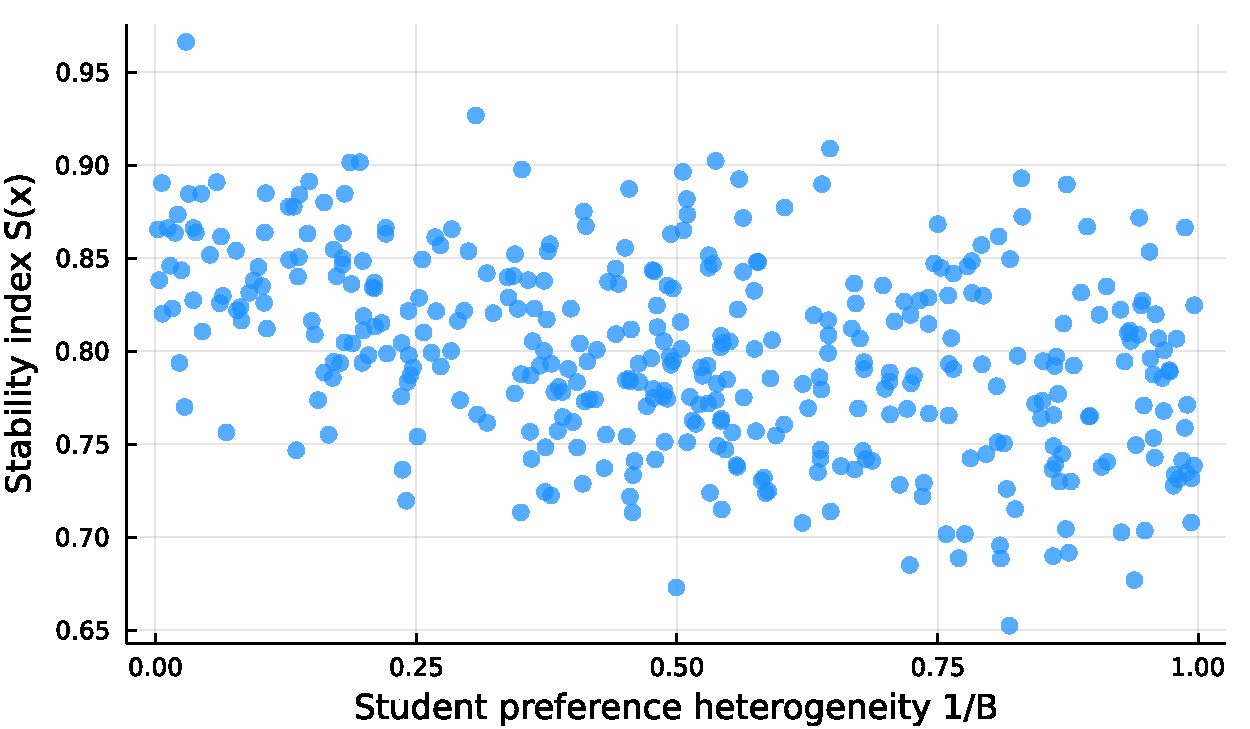
\includegraphics[width=0.95\textwidth]{./TwoSchoolModels/CombiPref-complementarity/heterogeneity-S.pdf}\end{center}
  \caption{(Heterogeneity experiment.) Effect of heterogeneity in students' risk preferences on the stability index $\bar S(x)$, a measure of the equilibrium's robustness to envy. Risk parameters $t_i$ were drawn from a $\operatorname{Beta}(B, B)$ distribution for 500 markets. 108 markets failed to converge to an equilibrium.}
\end{figure}

\begin{figure}[h!]
  \begin{center}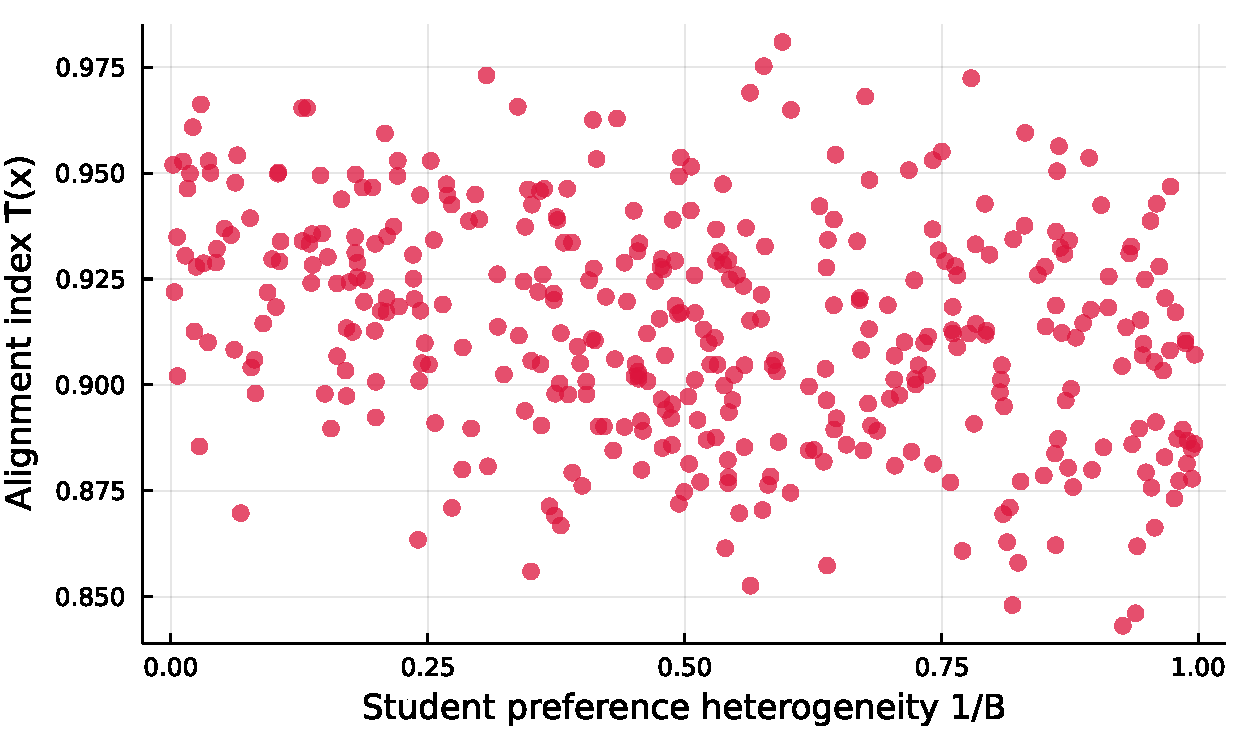
\includegraphics[width=0.95\textwidth]{./TwoSchoolModels/CombiPref-complementarity/heterogeneity-T.pdf}\end{center}
  \caption{(Heterogeneity experiment.) Effect of heterogeneity in students' risk preferences on the alignment index $\bar T(x)$, a measure of the selective school's ability to approximate its ideal entering class using the subset of students who apply. }
\end{figure}

\begin{figure}[h!]
  \begin{center}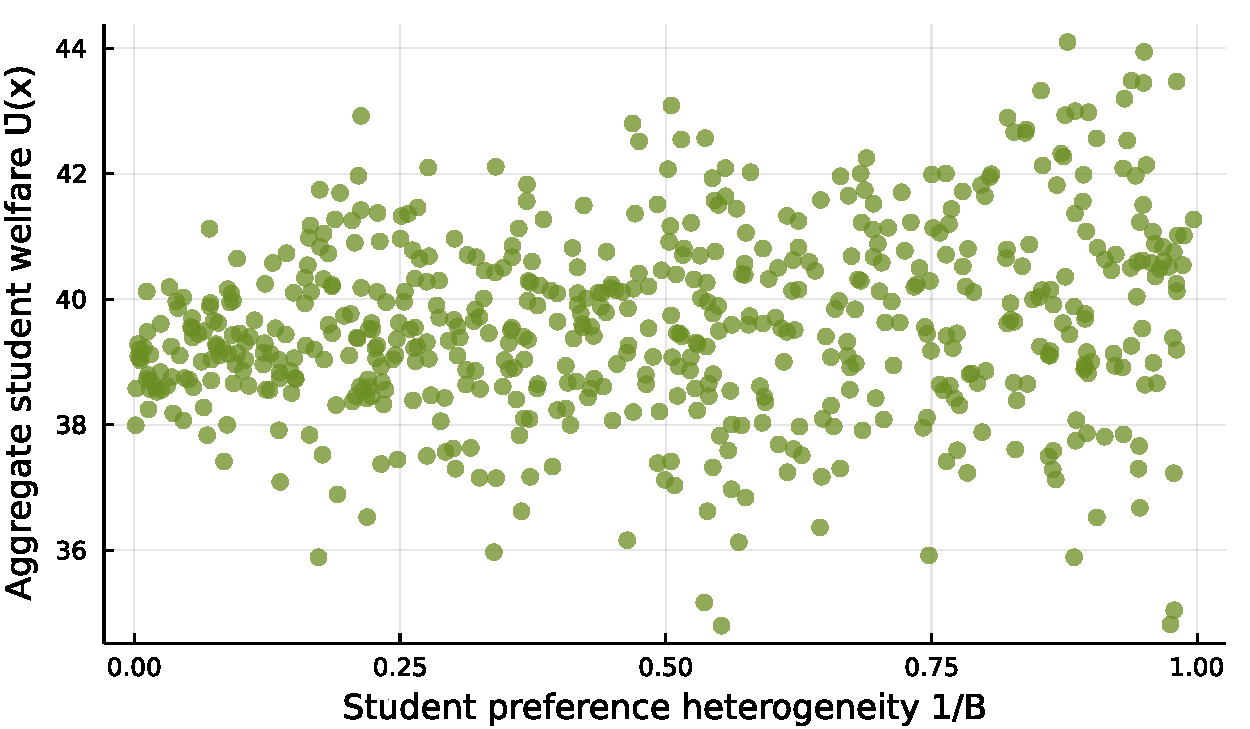
\includegraphics[width=0.95\textwidth]{./TwoSchoolModels/CombiPref-complementarity/heterogeneity-U.pdf}\end{center}
  \caption{(Heterogeneity experiment.) Effect of heterogeneity in students' risk preferences on the aggregate student welfare $\bar U(x)$.}
\end{figure}

\begin{figure}[h!]
  \begin{center}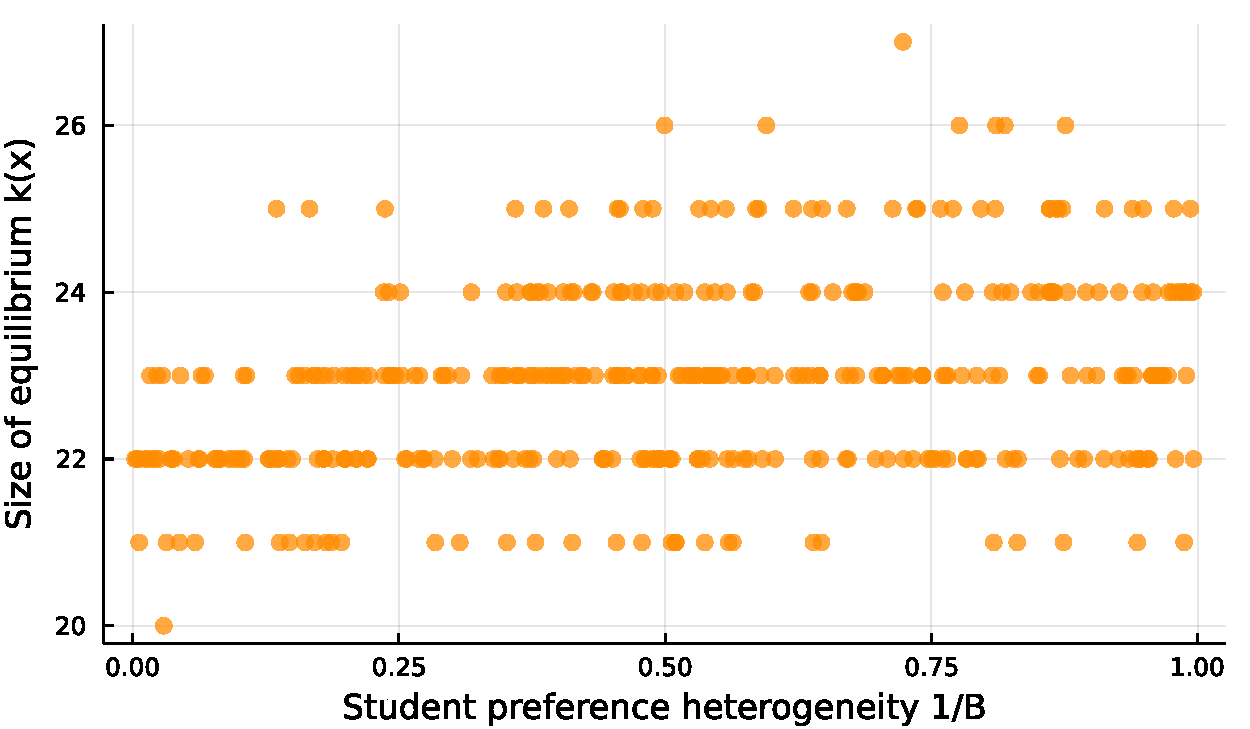
\includegraphics[width=0.95\textwidth]{./TwoSchoolModels/CombiPref-complementarity/heterogeneity-k.pdf}\end{center}
  \caption{(Heterogeneity experiment.) Effect of heterogeneity in students' risk preferences on the size of the equilibrium $\bar k(x)$.}
\end{figure}

\begin{figure}[h!]
  \begin{center}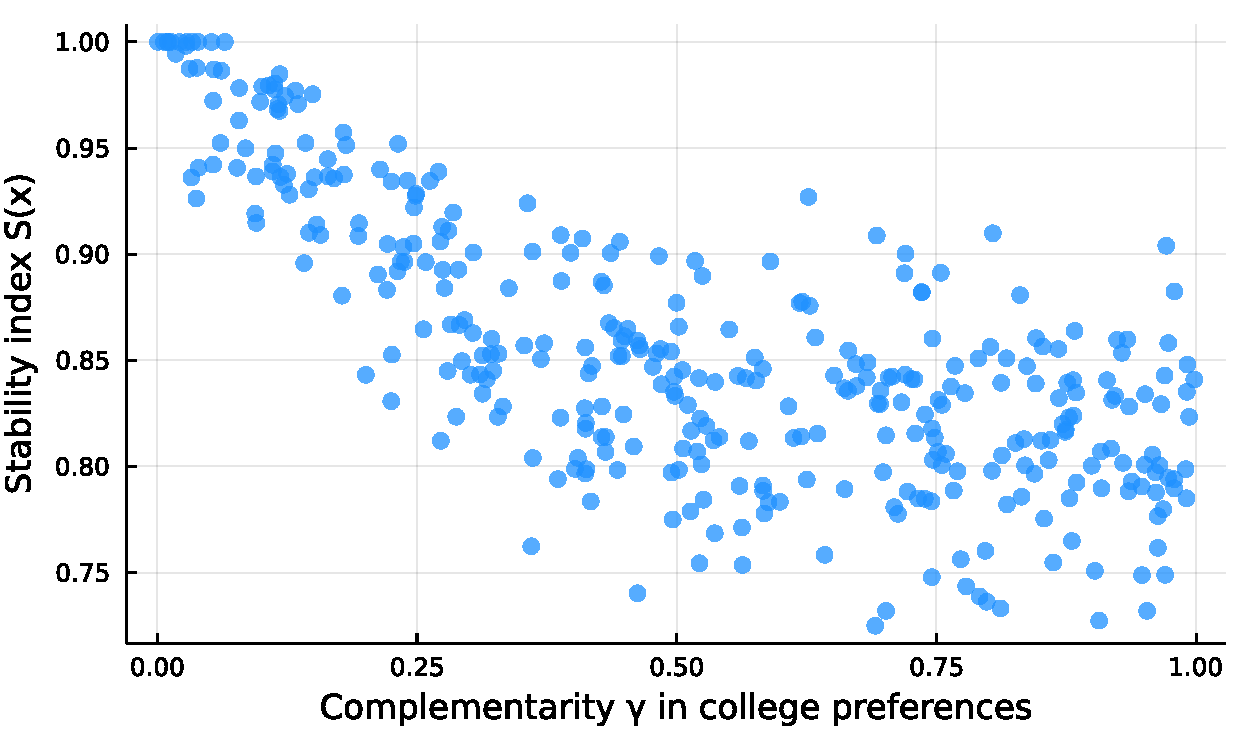
\includegraphics[width=0.95\textwidth]{./TwoSchoolModels/CombiPref-complementarity/complementarity-S.pdf}\end{center}
  \caption{(Complementarity experiment.) Effect of nonlinearity in the selective school's objective function on the stability index $S(x)$, a measure of the equilibrium's robustness to envy. 500 random markets with $\gamma \sim \operatorname{Uniform}(0, 1)$ were simulated. 142 markets failed to converge to an equilibrium. }
\end{figure}

\begin{figure}[h!]
  \begin{center}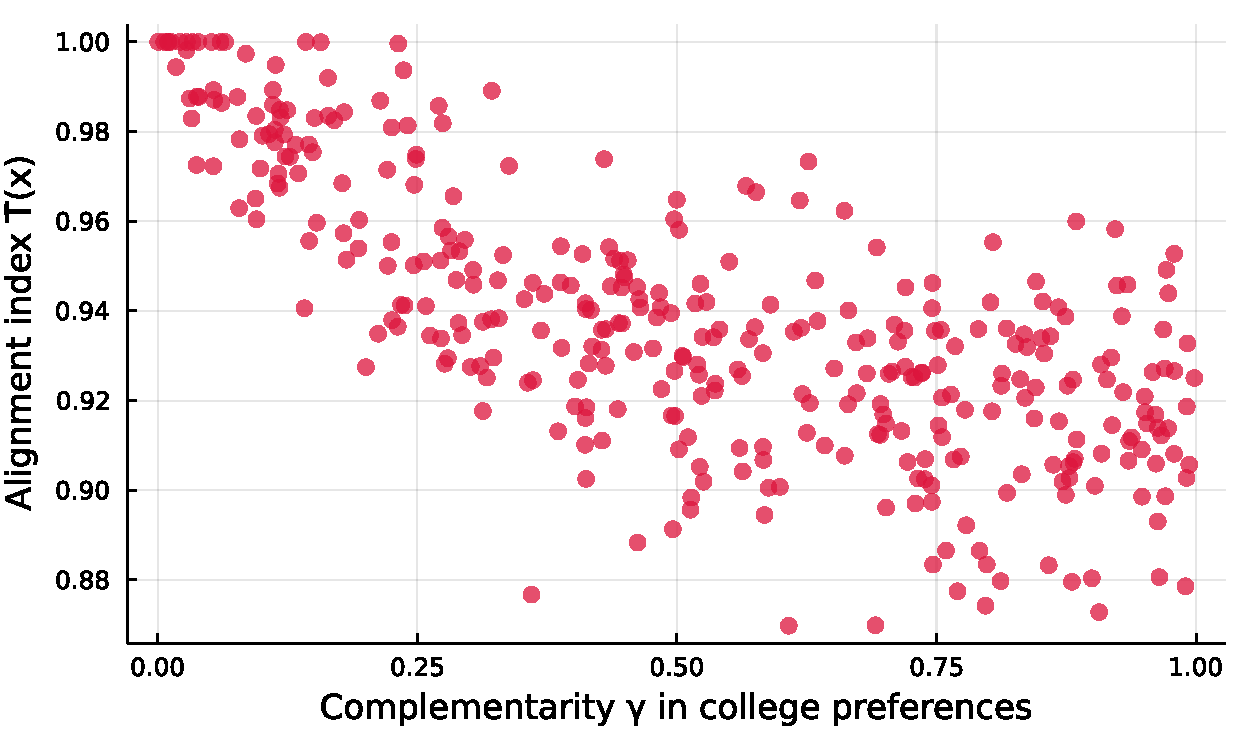
\includegraphics[width=0.95\textwidth]{./TwoSchoolModels/CombiPref-complementarity/complementarity-T.pdf}\end{center}
  \caption{(Complementarity experiment.) Effect of nonlinearity in the school's objective function on the alignment index $\bar T(x)$, a measure of the selective school's ability to approximate its ideal entering class using the subset of students who apply.}
\end{figure}

\begin{figure}[h!]
  \begin{center}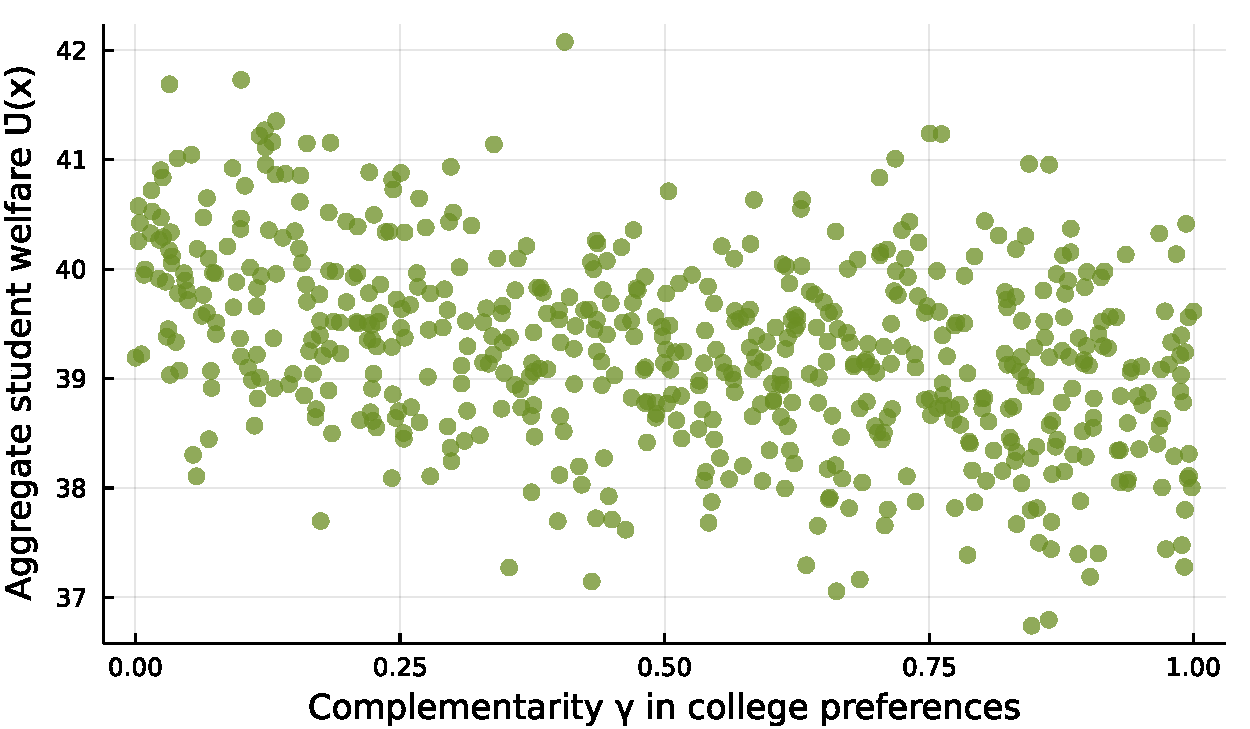
\includegraphics[width=0.95\textwidth]{./TwoSchoolModels/CombiPref-complementarity/complementarity-U.pdf}\end{center}
  \caption{(Complementarity experiment.) Effect of nonlinearity in the school's objective function on the aggregate student welfare $\bar U(x)$. }
\end{figure}

\begin{figure}[h!]
  \begin{center}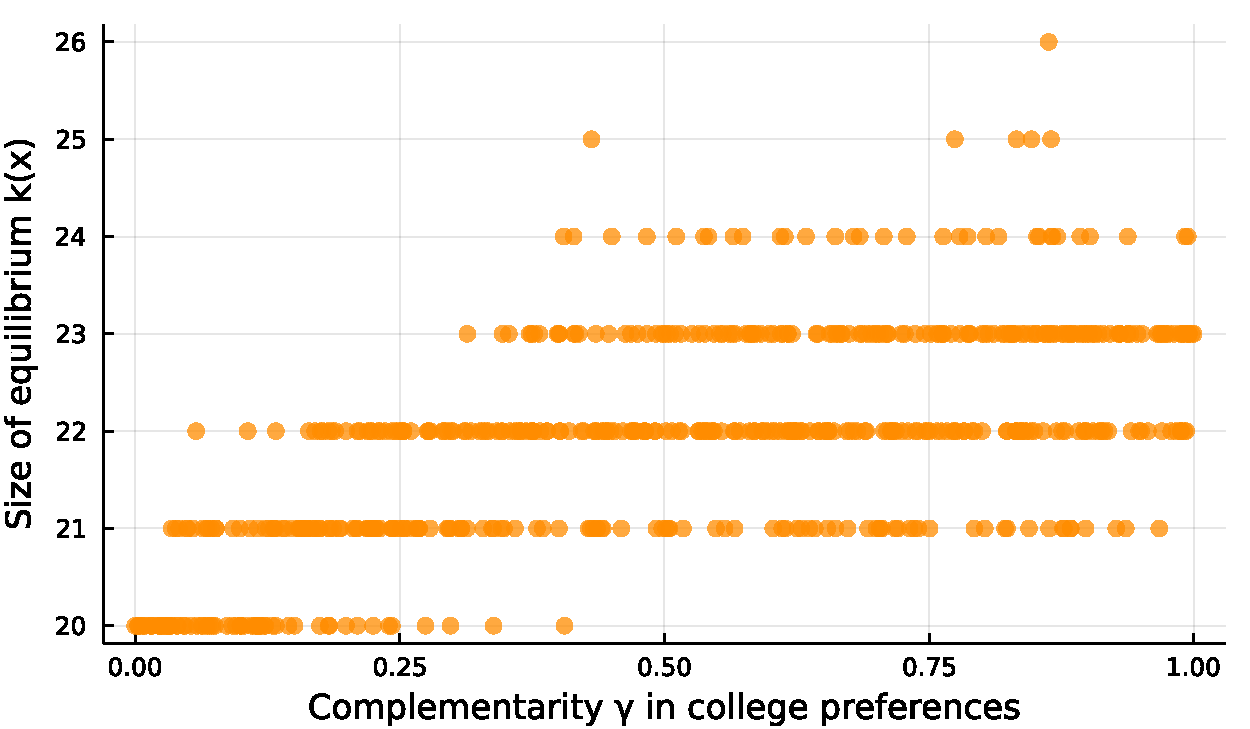
\includegraphics[width=0.95\textwidth]{./TwoSchoolModels/CombiPref-complementarity/complementarity-k.pdf}\end{center}
  \caption{(Complementarity experiment.) Effect of nonlinearity in the school's objective function on the size of the equilibrium $\bar k(x)$.}
\end{figure}



\pagebreak
\ifEN \section{References} \else \section{참고문헌} \fi
\noindent

\parskip 0em
\leftskip 2em
\parindent -2em
Budish, Eric. 2011. ``The Combinatorial Assignment Problem: Approximate Competitive Equilibrium from Equal Incomes.'' \emph{Journal of Political Economy} 119 (6): 1061--1103. \url{https://doi.org/10.1086/664613}. 

Dantzig, George B. 1957. ``Discrete-Variable Extremum Problems.'' \emph{Operations Research} 5 (2): 266--88.

Fisher, Marshall, George Nemhauser, and Laurence Wolsey. 1978. ``An analysis of approximations for maximizing submodular set functions—I.'' \emph{Mathematical Programming} 14: 265--94. 

Fredman, Michael Lawrence and Robert Tarjan. 1987. ``Fibonacci heaps and their uses in improved network optimization algorithms.'' \emph{Journal of the Association for Computing Machinery} 34 (3): 596--615.

Fu, Chao. 2014. ``Equilibrium Tuition, Applications, Admissions, and Enrollment in the College Market.'' \emph{Journal of Political Economy} 122 (2): 225--81. \url{https://doi.org/10.1086/675503}. 

Garey, Michael and David Johnson. 1979. \emph{Computers and Intractability: A Guide to the Theory of NP-Completeness.} New York: W. H. Freeman and Company. 

Othman, Abraham, Eric Budish, and Tuomas Sandholm. 2010. ``Finding Approximate Competitive Equilibria: Efficient and Fair
Course Allocation.'' In \emph{Proceedings of 9th International Conference on Autonomous Agents and Multiagent Systems.} New York: ACM. \url{https://dl.acm.org/doi/abs/10.5555/1838206.1838323}.

Rozanov, Mark and Arie Tamir. 2020. ``The nestedness property of the convex ordered median location problem on a tree.'' \emph{Discrete Optimization} 36: 100581. \url{https://doi.org/10.1016/j.disopt.2020.100581}.

% p. 70: FPTAS for knapsack, should work for Ellis's problem
Vazirani, Vijay. 2001. \emph{Approximation Algorithms.} Berlin: Springer. 

\end{document}  

